% !TEX root = ../../thesis.tex

\cleartoleftpage
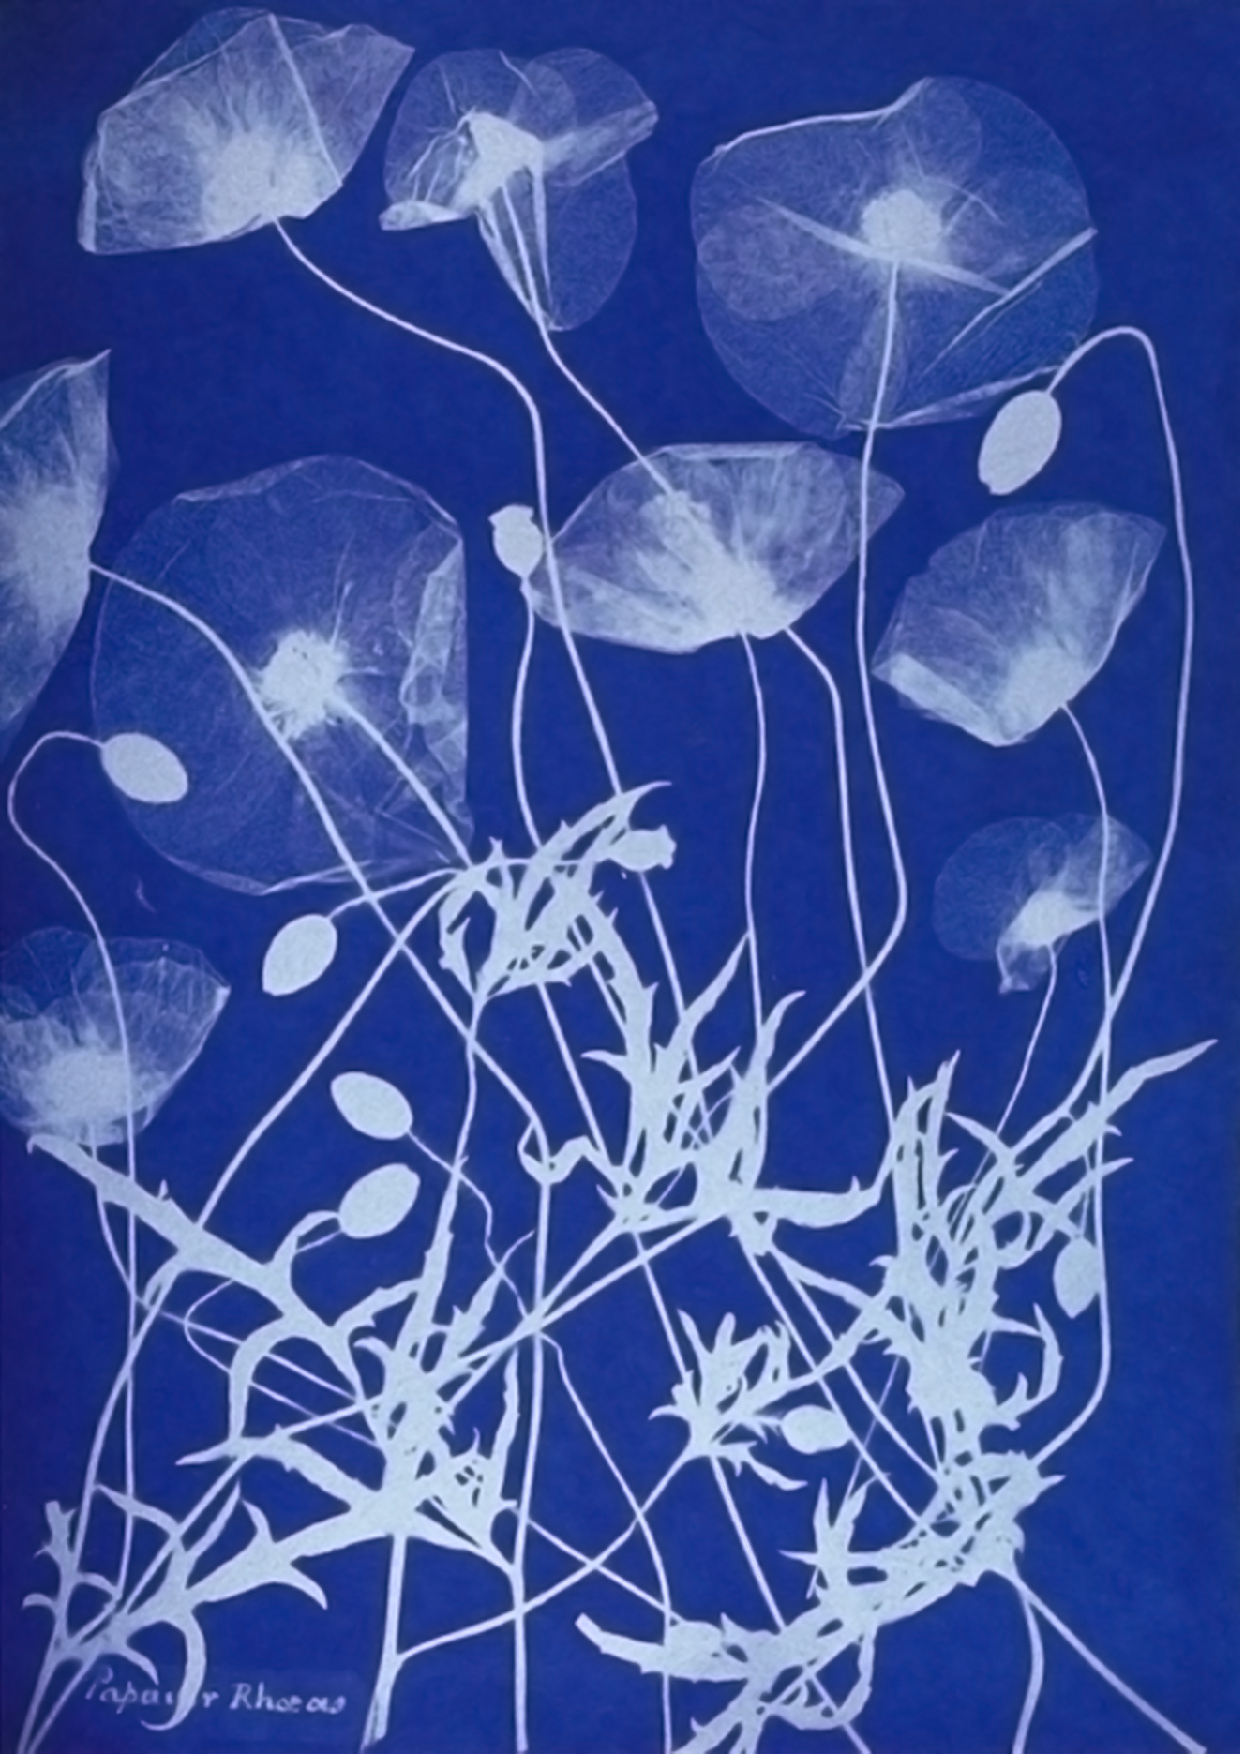
\includepdf{../media/chapter_illustration/papaver_rhoeas}
\chapter{The Poppy development} % (fold)


\section{Introduction} % (fold)

\begin{figure}[tb]
\centering
    \subfloat[][Nao]{\label{fig:nao_platform}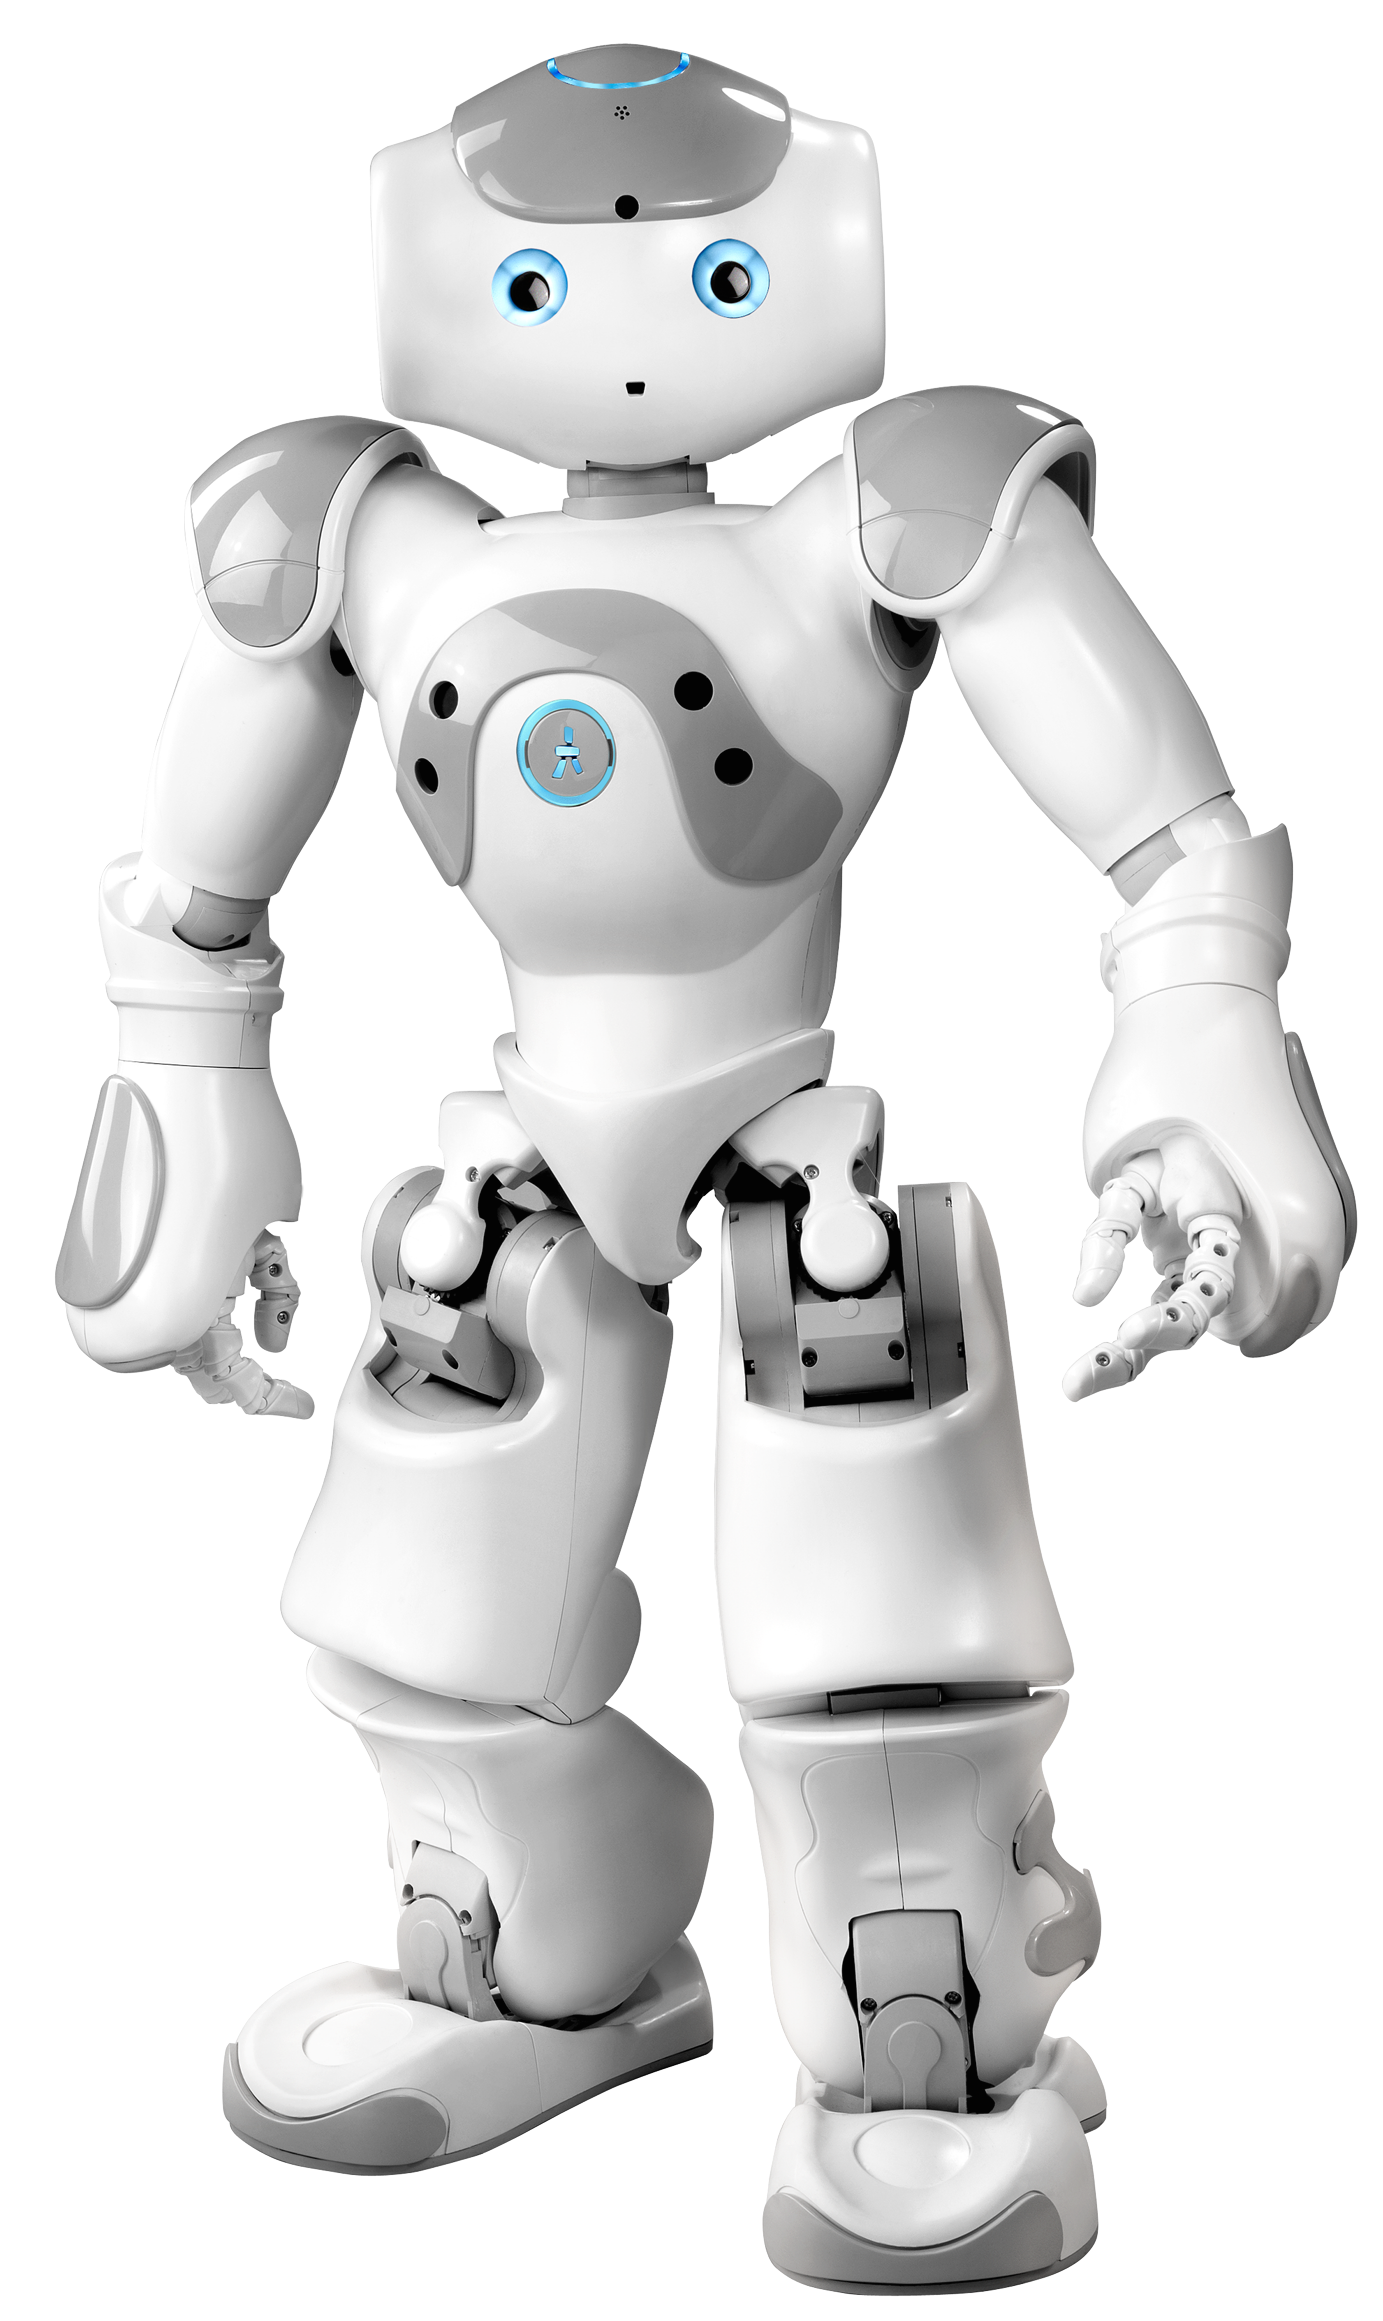
\includegraphics[height=5cm]{nao_face.png}}
    \hfil
    \subfloat[][Darwin-Op]{\label{fig:darwin_platform}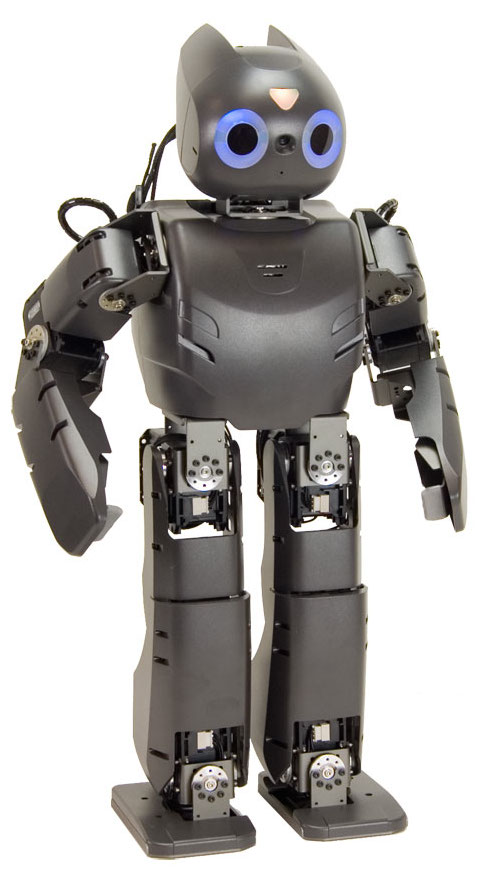
\includegraphics[height=5cm]{darwin_op_face.jpg}}
    \hfil
    \subfloat[][Acroban]{\label{fig:acroban_platform}\includegraphics[height=5cm]{acroban_wout_background.jpg}}
    \caption{None of the existing platforms in 2012 were suitable for exploring the role of morphology. Nao was impossible to modify. Darwin Op and Acroban used aluminium parts that are really difficult and expensive to produce.}
    \label{fig:2012_Humanoids}
\end{figure}

In 2012, when we started this project, none of the existing humanoid platforms were suitable for exploring the role of morphology. There were two kinds of platform. On one hand commercial robots that are rather easy to use and accessible but with a static and frozen morphology. On the other hand, prototype robots produced in labs to address specific experimentation needs, studying interesting morphologies but complicated to use and impossible to reproduce outside the lab. In both cases, only a few are open source, limiting hacks, extensions or modifications of their morphologies even further.




In the Flowers Lab, we had both kinds of robot. We used Nao (see \figurename~\ref{fig:nao_platform}) to study human robot interaction (REF PIERRE cadeau). It was really convenient for use by researchers who are not interested in hardware issue since they are addressing more high-level research challenges. Yet such a platform is limited as it is not possible to modify the robot if it is not strictly adapted to our experiment. For example, back at this time the Nao camera was not efficient, with a closed field of view and a slow framerate. We have difficultly achieved 5 frames/seconds. Although we had the necessary skills to hack Nao and change the camera to fit our needs, its hardware is not designed to be changed. Improving the vision performance would only be possible with the addition of an external camera on the Nao head which would ruin the user experience. In addition, it would have been interesting to explore how the camera parameters (FOV, framerate, resolution...) can change the user experience but again, it is not possible with this robot.



We also used Acroban (see \figurename~\ref{fig:acroban_platform}) designed by Olivier Ly~\cite{Ly2010}. It is a handcrafted humanoid platform created to explore certain morphological properties, especially compliance, with the aim of achieving dynamic locomotion and playful physical human robot interaction.
While it actually allows modification of its is morphology, it is manufactured from aluminium mechanical parts, Robotis Dynamixel motors, scotch, and rubber bands cobbled together, and changing it requires lot of effort . The manufacture of aluminium parts required is especially complicated and requires either very good handiwork or a 3-axis CNC.

In addition, its use was quite complicated and while several researchers could have been interested by Acroban to study human robot interaction and social acceptance, it was not possible to use it without getting our hands dirty.
Finally, the material and manufacturing process make the platform non-stationary. Even if a lab manages to reproduce it, there is a high probability that the physical properties will not be the same. Therefore, the diffusion and the reproducibility of results are limited.


A last alternative would be the use of Darwin Op robot (see \figurename~\ref{fig:darwin_platform}) which is both open source and easily accessible (Robotis sells it already assembled for \$10K), yet as Acroban its hardware consists of manufactured metal parts making its morphology very difficult and expensive to modify (see section REF for more details). Moreover, , even if Darwin is open source and very popular, to our knowledge its morphology has never be modified by the research community.

Thus one of the main goals was to successfully design a humanoid robot which can merge the advantages of both kind of robot, i.e. simple, accessible, reproducible and allowing to easily change and hack its morphology for scientific experiments that can be both customized and shared.


\subsection{An experiments-proof robot} % (fold)

Most researchers can attest to the difficulty and frustration faced while conducting robotic experimentation in the real world. We are challenged daily by bugs, technical issues, unpredicted events and side effects. While a bug in software can be fixed, an error with a hardware platform can cause damage to the robot and postpone the results of an experiment by several weeks.

Therefore many researchers in robotics avoid technical issues associated with the real world experimentation by using simple models and physical simulation. But the real world is extremely more complex and richer than the virtual one.
Some high-level behaviour experiments are conducted in simulators based on the hypothesis that real-world constraints are not relevant, yet it is really certain?
Indeed, while the real world constitutes a lot of constraints, it is also rich in complex physical effects (gravity, friction, inertia), which should be taken into consideration and could be very useful if interacting with the agent.

As we saw in the related work (chapter~\ref{REF}), the emergence of complex behaviours appears thanks to the interaction between the real world and simple robotic systems. We cannot program behaviour because behaviour is the result of interaction  between the program and the real world. Thus we cannot design behaviour without the ecological niche of the robot~\cite{Steels1991emergence}.

While using simulators can be helpful as a first step to design robots, it appears incomplete when showing results on the role of morphology without real world experimentation.
Therefore, when one wants to study the role of morphology on robot behavior, being able to explore it in the real world is of paramount importance. Unfortunately, current tools make the experimental step really hard to achieve for researchers.

Throughout our work on building cognitive and developmental learning algorithms, we have experienced these issues, especially while building and using Acroban~\cite{Ly2010} and during the Ergo robot experience (see section~\ref{REF}). Much time has been spent debugging non-robust technologies but it has been very instructive for understanding those that are efficient and those that should be avoided.
Therefore Poppy has been designed based on the background experience we have acquired building using robots acting in the real world.

\begin{description}
    \item[Robustness and Safety:] Demanding and lengthy real-world experimentation necessitates that the robot be robust and safe. It should be able to sustain experiments and fall down without easily breaking. At the same time, one should ensure that physical interaction with the robot is safe for humans.
    \item [Precision, stationary:]Experiments should be repeatable, implying that the robot properties should be stationary.
    \item [Breakable, repairable:] Breaking should not be costly and the robot should be easily repairable.
    \item [Transportable:] To allow for experiments in natural environments, possibly involving interaction with non-technical humans, the robot should be transportable outside the laboratory.
    \item [Easy and fast to duplicate:]If the robotic platform is to be reused  in this way, it must be easy and fast to duplicate.
    \item [Affordable:] To ensure widespread use, a key factor is to keep the cost of the platform relatively low. The more labs can be involved, the greater the scientific impact.
\end{description}


\subsection{Overview} % (fold)

To respond to this need we created Poppy,  the first complete 3D printed open-source and open-hardware humanoid robot (see \figurename~\ref{fig:poppyv0.1_overview}). Its 3D printed skeleton and its Arduino-based electronics are open-hardware (Creative Commons). Its software is open-source (GPL V3), and allows programming beginners as well as advanced roboticists to control the robot in Python thanks to the PyPot library. Its motors are common and widely used off-the-shell Robotis actuators, and allow for compliant control and soft physical human-robot interaction. Poppy presents an original mechanical structure that permits to obtain a light structure with 3.5kg for 84cm height.
Its current morphology takes insight from the human functional morphology: large number of articulation (25 motors), the limbs respect human proportions, it has five articulation in the trunk and its thigh is bended by a $6\deg$ angle similar to the human.

Underactuated

Discuss the size of the robot

\begin{figure}[tb]
    \begin{center}
        \includegraphics[width=0.95\linewidth]{poppy-overview.pdf}
    \end{center}
    \caption{}
    \label{fig:poppyv0.1_overview}
\end{figure}


\section{Explore morphological variants} % (fold)

The whole structure must be easily reconfigurable both for repairing or hacking purposes. This mean the process to replace a Poppy's parts must be simple, low-cost and not require time or special tooling. Also, in order to have a real impact in the open hardware community, special attention is given to the modularity and the reusability of our technological bricks.
Poppy is fully modular (mechanic, electronic, software) allowing to freely explore and modify Poppy's body.
Its modularity and the use of 3D printing make Poppy highly hackable. It can be easily adapted to particular experimental setups.


\subsection{3D printed parts} % (fold)

We introduced for the first time the use of 3D printed mechanical parts in our work when we built the ergo-robot installation (Aout 2011 - see Chapter REF). The result was impressive as the parts were robust, precise, low-cost and fast to produce. Very convinced by this technology and desiring to be free to explore the robot morphology, we decided to build the whole mechanical structure of Poppy based on 3D printing techniques.

\subsubsection{Technique used} % (fold)

Several 3D techniques exist and were presented in the related work (see section REF). The Stereo-Lithography\footnote{This technique relies on a photosensitive monomer resin which forms a polymer and solidifies when exposed to ultraviolet (UV) light.} (SLA) is very precise yet the material is not well adapted to support mechanical constraints.

Alternatively, we can use Fused Deposition Modeling\footnote{The FDM technique relies on melting and selectively depositing a thin filament of thermoplastic polymer (ABS - PLA) in a cross-hatching fashion to form each layer of the part.} (FDM), which has the great advantage of being very low cost (2000\$ for the printer + 40\$/kg of material) and therefore accessible directly in the labs. The part produced are good yet the finish is not perfect and require to be reworked by hand. Also the process create non uniform part, less resistant on one axis. Above all the FDM printers have low reliability leading to a large number of printing fails. Nevertheless low-cost FDM printers are really useful when we just want to produce first instance or single time use parts.

So we preferred the use of Selective Laser Sintering (SLS)\footnote{The process uses a high power (25-50W) CO2 laser beam which melts and fuses fine powdered material spread on a layer.}. This 3D printing process allows the production of almost any shape without constraint. In addition, the price of the part depends on the total size and not on the complexity of the shape. This permits the production of very optimized shapes without increasing the total price of the robot. Moreover the use of polyamide material produces high quality part with very good mechanical properties uniform, lightweight, flexible and robust.

The table~\ref{tab:materials} compares mechanical properties of polyamide with classic metallic materials. We can notice the relatively good properties of the polyamide material. The young modulus represents the stiffness of the part. The polyamide one has a very low young modulus meaning it is very flexible while keeping a correct yield strength and a very low density.

\begin{table}[h]
    \centering
    \begin{tabularx}{0.8\linewidth }{l X X X}
        Material & Mass Density $\rho$ ($kg/m^3$) &  Yield strength $\sigma$~($MPa$) & Young Modulus $E$($GPa$)\\
        \hline
        Polyamide & $930$ & $49$ & $1.65$\\

        Aluminum & $2700$ & $200$ & $70$\\

        Steel & $7500-8000$ & $350$ & $200$\\

        Titanium & $4500$ & $1200$ & $114$\\

    \end{tabularx}

    \caption{Comparison of material properties.
    The Young modulus represents the stiffness of the material while the yield strength corresponds to the maximal stress tolerable before plastic deformation.}
    \label{tab:materials}
\end{table}

A SLS printer is much too costly for a labs, yet sourcing the production to external company\footnote{\url{http://i.materialise.com/}} is really easy\footnote{In most cases, the company offers automatic scalable orders through on-line platform} and relatively low cost\footnote{Printing all the parts to build a Poppy costs about 1200\texteuro HT.}

\subsection{Exploring morphological variants} % (fold)
The 3D printing is a central aspect in Poppy to permit the exploration of morphological variant. Because it is now cheap and easy to produce custom part, we can quickly change the morphology of Poppy.

To do so, it is only needed to change the desired parameter in the source file and reprint the part. And because Poppy is open source, anyone has access to the source files and can freely change the parameters he wants.

\begin{figure}[h]
    \begin{center}
        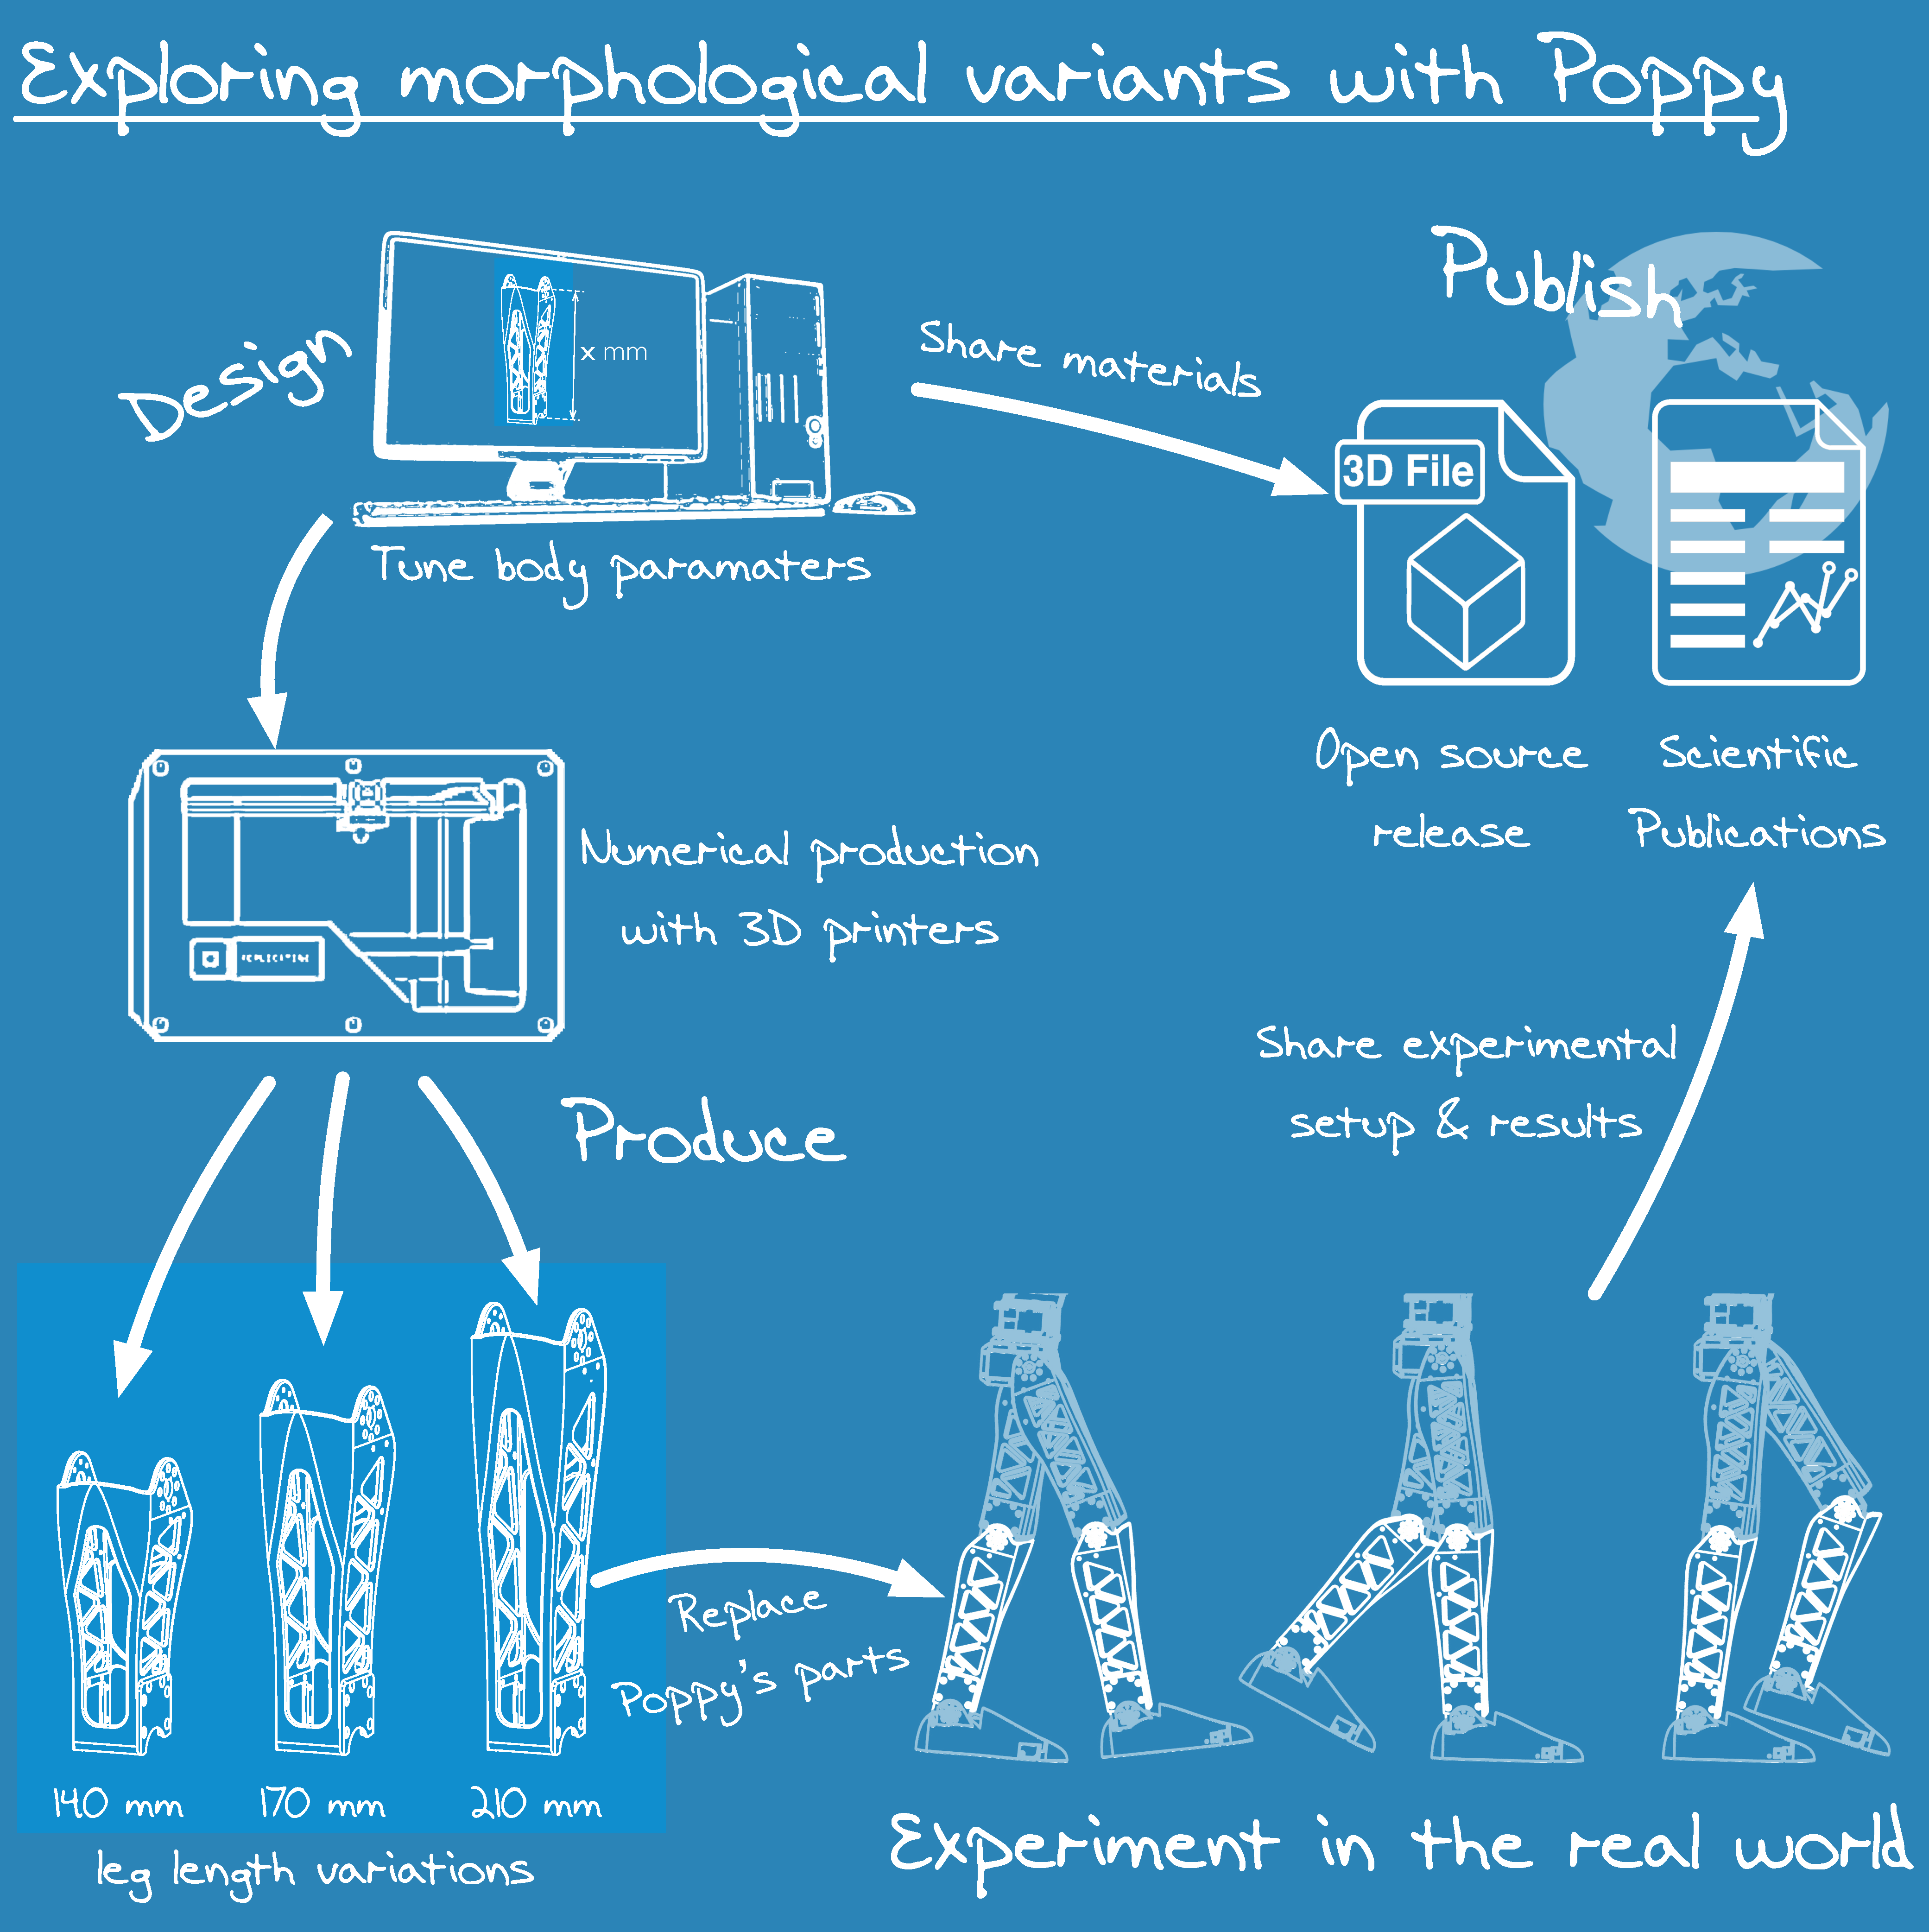
\includegraphics[width=\linewidth]{morpho_variation.pdf}
    \end{center}
    \caption{Caption here}
    \label{fig:figure1}
\end{figure}


Moreover, 3D printing does not only permit to change the shape of a part, it can actually produce it with different material. In particular, Direct Metal Laser Sintering (DMLS) - very similar with the SLS process - permits to produce the same parts using steel\footnote{http://i.materialise.com/materials/stainless-steel} and titanium\footnote{\url{http://i.materialise.com/materials/titanium}}. It is therefore possible to explore at the same time mechanical properties (e.g. flexibility, density) and shapes.


\subsection{Scalable actuation} % (fold)

As explained in the chapter REF, the chose methodology relies on the all-in-one Robotis actuator. They are really convenient to use as they directly embed drivers, encoders and communication bus. They are also quite powerful, robust and rather precise. This is done by the combination of Maxon motors, metal gearbox and precise magnetic rotation sensor (resolution: 0.1\textsuperscript{o}).

Also Robotis offers a range of motors with different actuation power (see \figurename~\ref{fig:dynamixel_powa}). They are different in size and power but their API remains the same and we can easily switch from one to another without neither changing the code nor the electronic integration. Yet, even if the size change, the foot-print keep the same pattern (see \figurename~\ref{fig:dynamixel_dimension}).

Poppy is designed with Solidworks, a parametric modeler which offers features like configurations\footnote{Configurations allow to create multiple variations of a part or assembly model within a single document. Configurations provide a convenient way to develop and manage families of models with different dimensions, components, or other parameters.}, which define set of parameters. Is it therefore possible to create for each part the configuration compatible with each motors, by setting the suitable parameter. The figure \figurename~\ref{fig:leg_configuration} shows an example with Poppy's leg. It just takes a couple of minute to transform a part designed for Dynamixel MX-28 to one compatible with Dynamixel MX-64. Then it is possible to switch from one to another with one click.

\begin{figure}[h]
    \begin{center}
        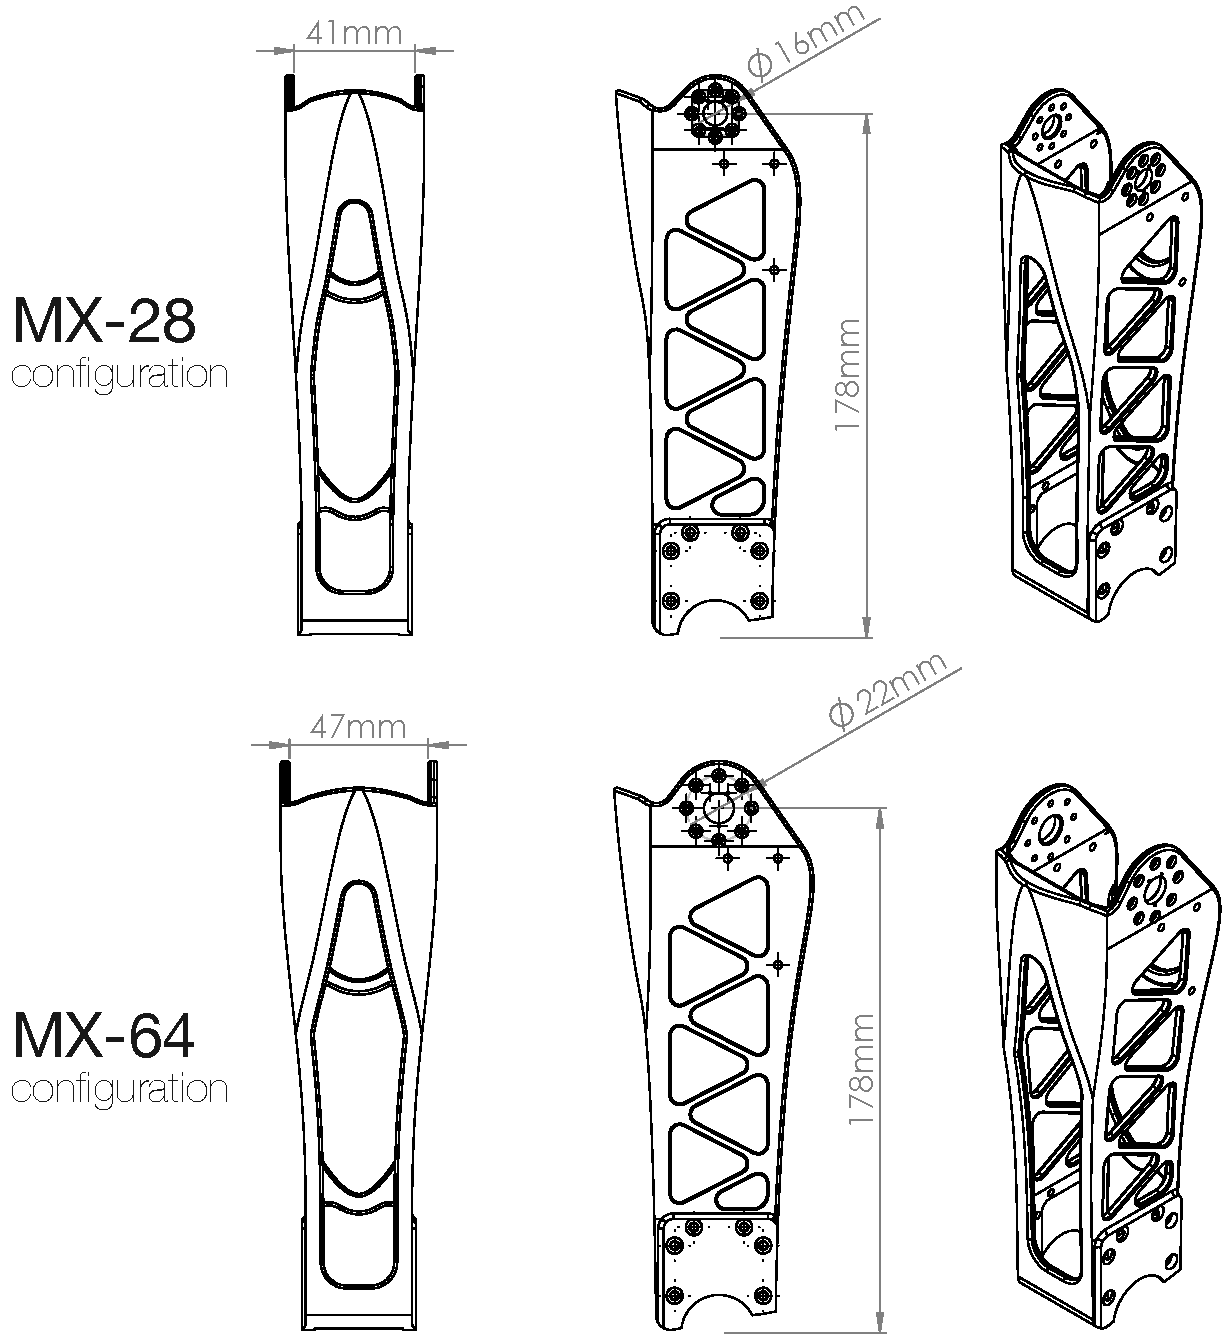
\includegraphics[width=\linewidth]{leg_configuration.pdf}
    \end{center}
    \caption{Poppy's leg configuration.}
    \label{fig:leg_configuration}
\end{figure}

On Poppy, most of the parts are already distributed with multiple configuration suitable for different motors power. It permits to scale the actuation power and introduce it also as an experimental - discrete - variable.


\subsection{Electronic} % (fold)

Unlike the mechanical parts, there is no quick and low-cost solution allowing to produce custom electronic yet.
However, exploring the morphology may also required varying the sensors space (e.g. number, type, properties, positions). As we explained in the chapter REF, we address this challenge through the use of the Arduino environment.

Arduino has developed both hardware and software allowing to create and program electronics systems very easily. Their boards have plenty of I/O pins (digital and analog) suitable to power and control almost any electronics components. Also these pins can be used to handle low-level communication such as UART, SPI and I2C, useful to plug sub-module (e.g. IMU, LCD Matrix, tactile interface and so on).
The software they developed abstract very well the complexity of low level control\footnote{we can turn a led on/off with just one line of code.} and communication\footnote{Using just printf-like functions we can communicate on serial bus.}. Therefore, it allows a wide variety and flexibility to extend the electronic system while keeping an ease of use adapted to non-expert audience.
In addition, Arduino has an growing community -already pretty big- which creates, shares and produces low-cost, various and multipurpose electronic components. Actually almost of kind of sensors have an Arduino version with ready-to-use hardware and software.

Being able to change easily change the morphology is a paramount importance in the Poppy project. Using Arduino-compatible architecture permits an electronic modularity, which allow to consider the sensory-motor space as an experimental variable (see chapter REF).



\section{Lightweight} % (fold)

Many humanoid robots use powerful motors often associated with highly accurate sensors. This has a cost, both in terms of weight and computation resources. Moreover, to ensure the accuracy of the sensory-motor space it is necessary to design very rigid mechanical parts. The whole structure obtained is powerful but very heavy and due to inertia not very agile.
In the Poppy platform, the lightness is very important both for dynamical properties and safety:
\begin{itemize}
    \item for a given actuation power, reducing the link mass reduce its inertia and permits to increase the agility and the responsiveness,
    \item make Poppy a platform easier to manipulate and transport outside the lab,
    \item make the robot safer for people as well as for itself when it fall (and it will definitely fall a number of times).
\end{itemize}

The lightness was achieved by combining low-power actuation and optimized structure. Indeed when combined, it creates a kind of virtuous circle where the reduction of the maximum torque reduces the strength on mechanical parts. Because less force intensity is applied, we can remove material from parts. Because we have a lighter mechanical structure we can reduce the actuation power required and so on.

Also using low-power actuation has several interesting points:

\begin{itemize}
    \item The actuation being the main cost of the robot (>60\%), using the least powerful motors significantly reduces the total cost of the robot.
    \item Low-power actuators allows a safer robot. Indeed, in case of programing error, the robot is not enough powerful to hurt someone or itself.
    \item on a research challenge aspect, it constraints the possible motions to the one requiring few strength so certainly more human-like.
\end{itemize}

Therefore Poppy was designed using the weaker and lightest motors i.e. MX-28\footnote{Robotis motors are quite heavy (72, 126 and 153g respectively for MX-28, MX-64 and MX-106) in comparison of the Futaba servo-motors, 20-50g for a comparable output torque see \url{http://www.futaba-rc.com/servos/brushless.html}}, excepted on few particular joints (such as hip) while the mass reduction of the mechanical parts were achieved by using truss design.

Truss are a well-known design technique from structural mechanics to create lightweight yet very robust structures. It is mainly used in civil engineering (see \figurename~\ref{fig:truss_bridges}) but can also be used in plane, which require lightness and strength resistance.

\begin{figure}[tb]
    \begin{center}
        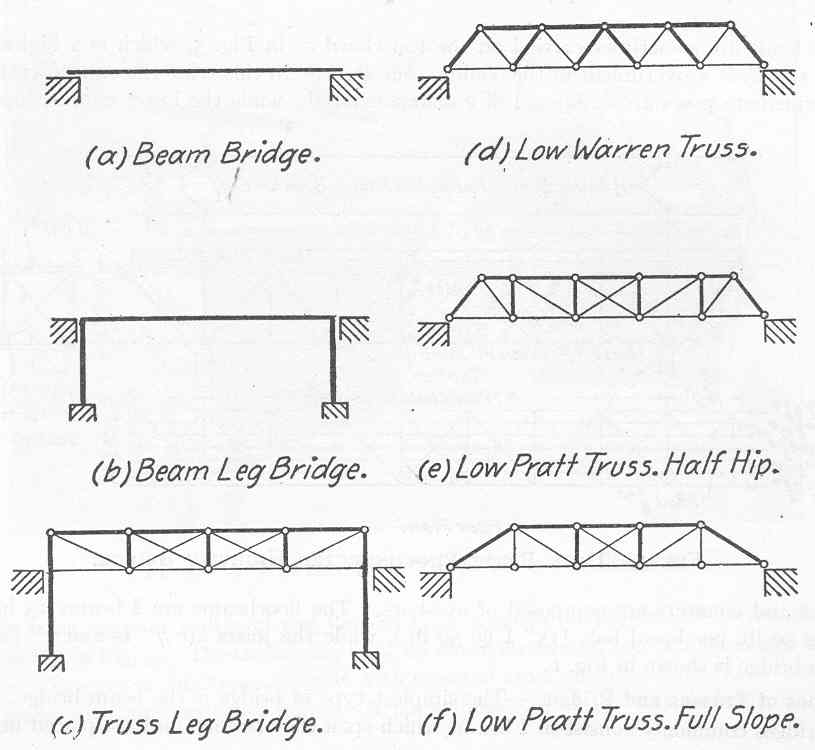
\includegraphics[width=0.6\linewidth]{truss_bridges.jpg}
    \end{center}
    \caption{Caption here}
    \label{fig:truss_bridges}
\end{figure}

The principle is based on beam theory and permit to increase the second moment of area a beam cross-section (see \figurename~\ref{fig:leg_section}), which is an important property in the calculation of deflection, main weakness of a long beam.

The second moment of area is computed as follow:

\begin{center}
    $I_x = \iint_s y^2 dxdy$

    $I_y = \iint_s x^2 dxdy$
\end{center}

where $s = dxdy$ is the surface integrated along the two axis of the cross-section surface. We can notice the  on each dimension varies with a quadratic factor meaning the variation is not linear. Therefore matter placed far away from the origin is much more effective to increase the second moment of area.
Thus the main idea is to remove -the no effective- matter at the center and place it on the rim. In truss structure, matter is assembled by linkage avoiding local deformation.

The \figurename~\ref{fig:leg_section} shows the comparative cross section of two beam with the same second moment of area value. More precisely, the \figurename~\ref{fig:Poppy_leg_section} is a cross section of Poppy's leg while the figure \figurename~\ref{fig:basic_leg_section} is a basic beam with a rectangular profile.

\begin{figure}[!h]
\centering
    \subfloat[][Section of the Poppy's leg]{\label{fig:Poppy_leg_section}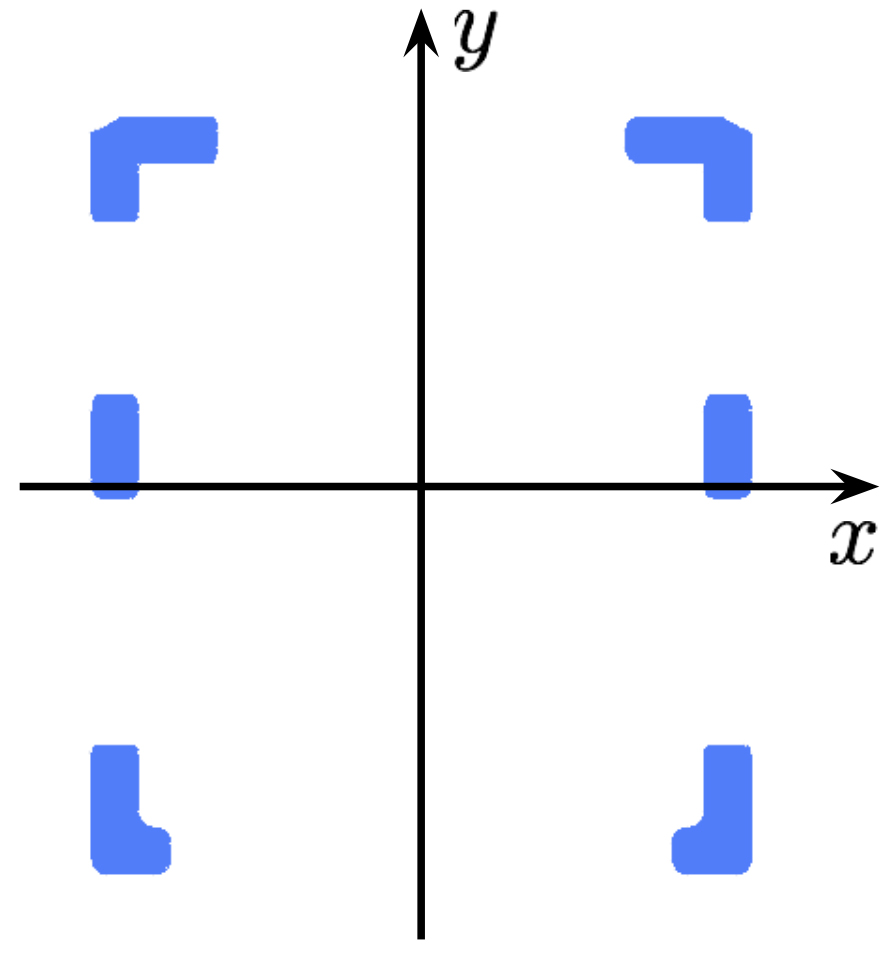
\includegraphics[height=4cm]{Poppy_leg_section.jpg}}
    \hfil
    \subfloat[][Equivalent rectangular section]{\label{fig:basic_leg_section}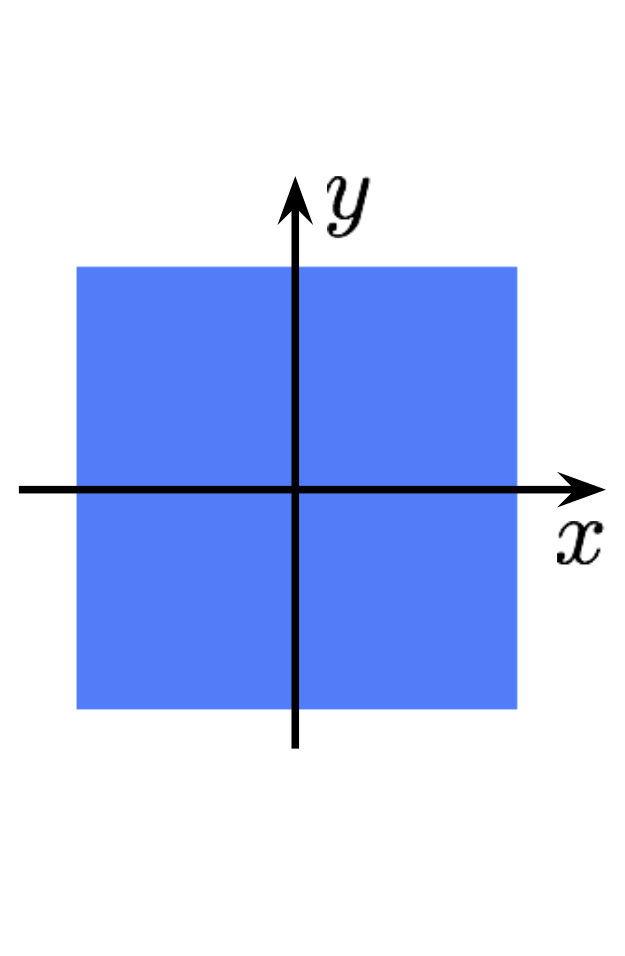
\includegraphics[height=4cm]{basic_leg_section.jpg}}
    \caption{}
    \label{fig:leg_section}
\end{figure}

It would require a section such as $b=27.72 mm$ and $h=27.59 mm$ for the rectangular to get the same quadratic momentum as the truss design (i.e. $I_x = 54.862 mm^4$ and $I_y = 53.260 mm^4$ measured with Solidworks).
Considering the length of the leg part (i.e. $190 mm$), the total mass would be equal to $142 g$ instead of $47 g$ for the actual leg. This corresponds to a reduction of 70\% of the mass.

\begin{figure}[!h]
\centering
    \subfloat[][]{\label{fig:poppy_arm_truss}\includegraphics[width=0.8\linewidth]{arm_truss.jpg}}


    \subfloat[][]{\label{fig:poppy_leg_truss}\includegraphics[width=0.8\linewidth]{leg_truss.jpg}}
    \caption{}
    \label{fig:poppy_truss_structure}
\end{figure}

All the limbs of Poppy are based on this structure and have been optimized using finite element analysis (FEA) to perform structural simulation and validate parts performance and safety factors.
Thanks to the use of this design on all Poppy's limbs (see \figurename~\ref{fig:poppy_truss_structure}), we managed to have -certainly- the most lightweight humanoid robot with 3.5kg relatively to its 83 cm height.






% \tikz[remember picture,overlay] \node[inner sep=0pt] at (current page.center){\includegraphics[width=\paperwidth,height=\paperheight]{Poppy_dimensions}};
% \clearpage
% \includepdf{../media/poppy/conception/Poppy_dimensions}


% \begin{figure}[p]
%     \begin{center}
%         \includegraphics[height=\textheight]{Poppy_dimensions.PDF}
%     \end{center}
%     \caption{Caption here}
%     \label{fig:figure1}
% \end{figure}





\section{Electronic architecture} % (fold)

TODO

\begin{figure}[tb]
    \begin{center}
        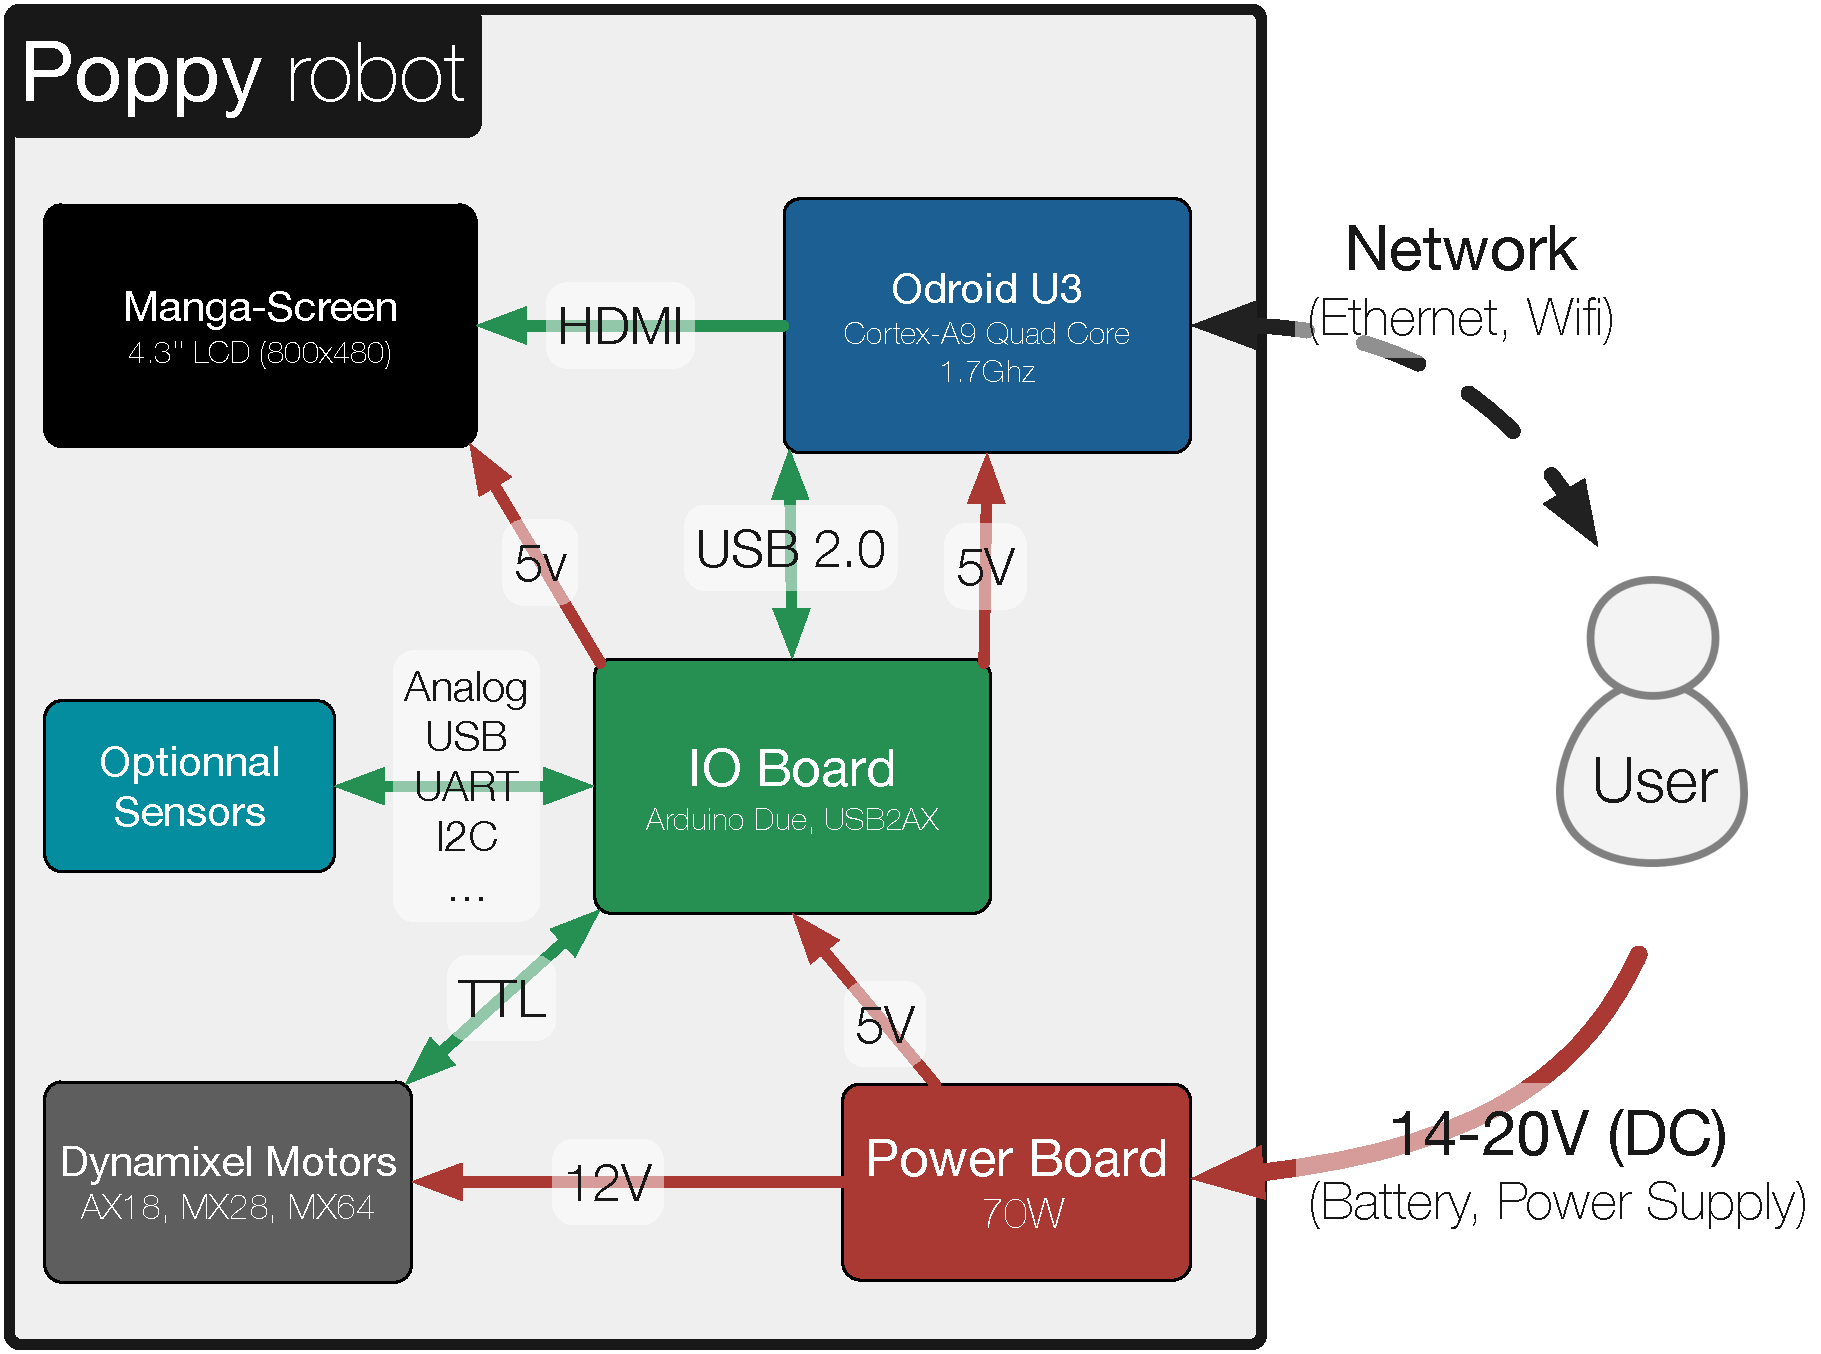
\includegraphics[width=\linewidth]{poppy_electro_archi_overview.pdf}
    \end{center}
    \caption{Caption here}
    \label{fig:figure1}
\end{figure}



\subsection{Poppy IO Board} % (fold)

To keep the spirit of the project described by its guidelines (see previous section REF), the electronic architecture has to be simple, easily reproducible, relatively low-cost and modular. Of course the performance of each components is very important and should be correctly dimensioned.

The first version of Poppy (beta) had a handmade electronics architecture, which required hacking several components before soldering them together. This design was not compliant with the design guidelines of Poppy (i.e. easy to use and to reproduce) and was actually the main reason Poppy was considered as a beta version. Recent work has been done toward the simplification and the reproducibility of the electronics part.

Yet the electronic integration is challenging. Indeed, because Poppy has 5 degrees of freedom in the torso, there is not enough room for all electronic components needed. Therefore we had to embed most of them in the head which raise a room problem but also a mass problem.

With the aim to offer easy-to-use modular electronics architecture and to make it fit in the head of Poppy, we decided to create a custom board. We could argue it makes more complex the diffusion of the platform while a custom board is too complex to be handmade and should therefore follows the industrialization process we are trying to avoid since the early age of the project. Nevertheless the makers revolution brings novel solutions to produce electronics. Indeed, there are now companies (such as CircuitHub\footnote{\url{https://circuithub.com}}), which offer scalable solution tools from 1 sample to a 10,000 batch. It is possible to upload our design and anyone can ask to make it produced. Of course ordering one part is more expansive but stay relatively low compare to the robot cost.

The board we design included the basic element needed both for the control of the robot and for its extensibility.


\begin{figure}[tb]
    \begin{center}
        \includegraphics[width=0.8\linewidth]{IO_Board.pdf}
    \end{center}
    \caption{Caption here}
    \label{fig:figure1}
\end{figure}


\subsubsection{Motor control} % (fold)
Robotis Dynamixel are normally controlled by the \emph{USB2Dynamixel} but we decided to replace it by USB2AX devices (see \figurename~\ref{fig:usb2ax}). The USB2AX is a small interface to control Dynamixel servomotors from a computer and designed by Nicolas Saugnier. It plugs into a USB port and has a 3-pin molex connector compatible with the robotis ones.

For the use in Poppy, these devices has several main advantages:
\begin{enumerate}
    \item They are a lot smaller than the standard USB2Dynamixel module (16x36mm instead of 35x90mm) (see \figurename~\ref{fig:USB2AX_vs_USB2Dxl}).
    \item They can endure a short-circuit between the DATA and power-supply wire.
    \item They have the sync\_read instruction to read a lot of information very fast, which is not a standard Dynamixel instruction. The USB2AX converts SYNC\_READ into multiple separate READ commands to get data from each servo, then sends back to the computer a single big packet containing all the data. This significantly decreases the effect of USB latency. A SYNC\_READ command reads the same registers in each servo.
    \item It is open source so we can extend or adapt this solution to our needs.
\end{enumerate}

\begin{figure}[tb]
\centering
    \subfloat[][]{\label{fig:usb2ax_dongle}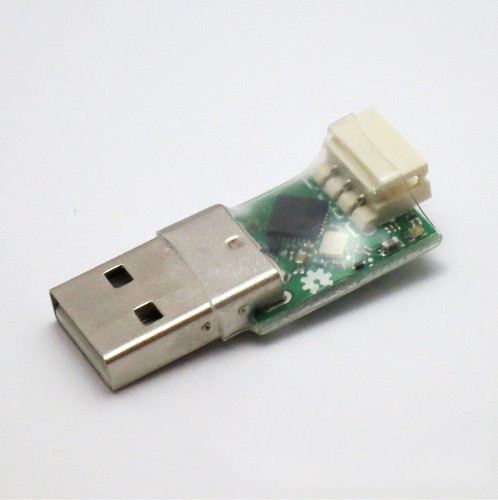
\includegraphics[height=5.5cm]{usb2ax.jpg}}
    \hfil
    \subfloat[][]{\label{fig:USB2AX_vs_USB2Dxl}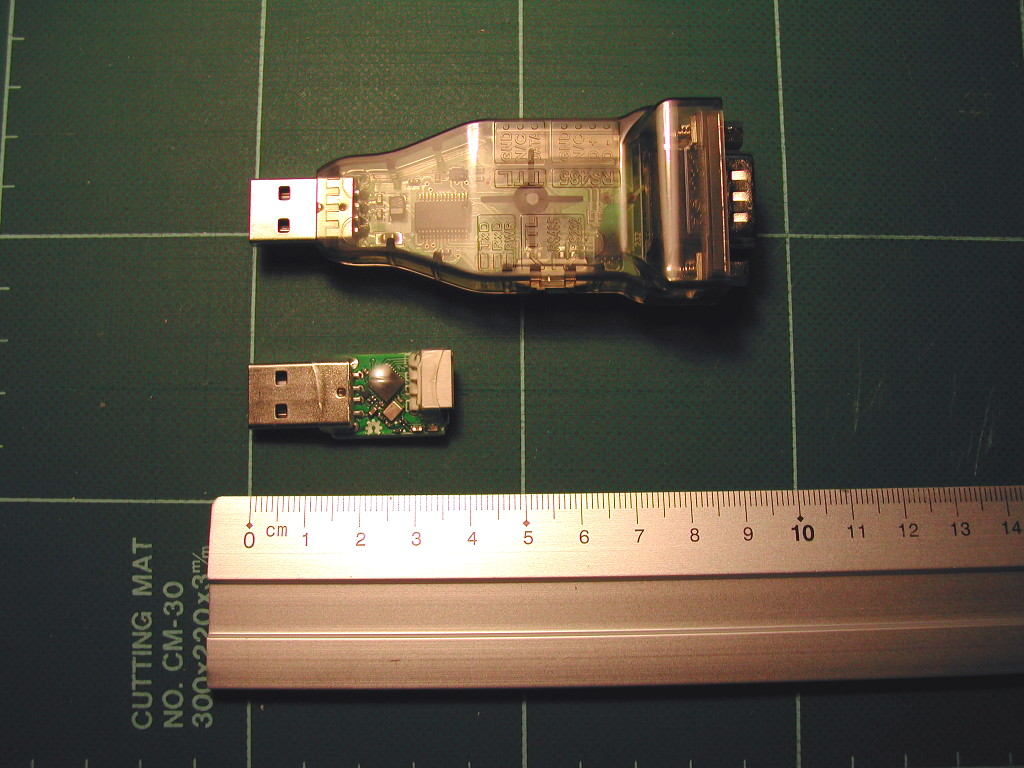
\includegraphics[height=5.5cm]{USB2AX_vs_USB2Dxl.jpg}}\\
    \caption{}
    \label{fig:usb2ax}
\end{figure}

\begin{figure}[tb]
    \begin{center}
        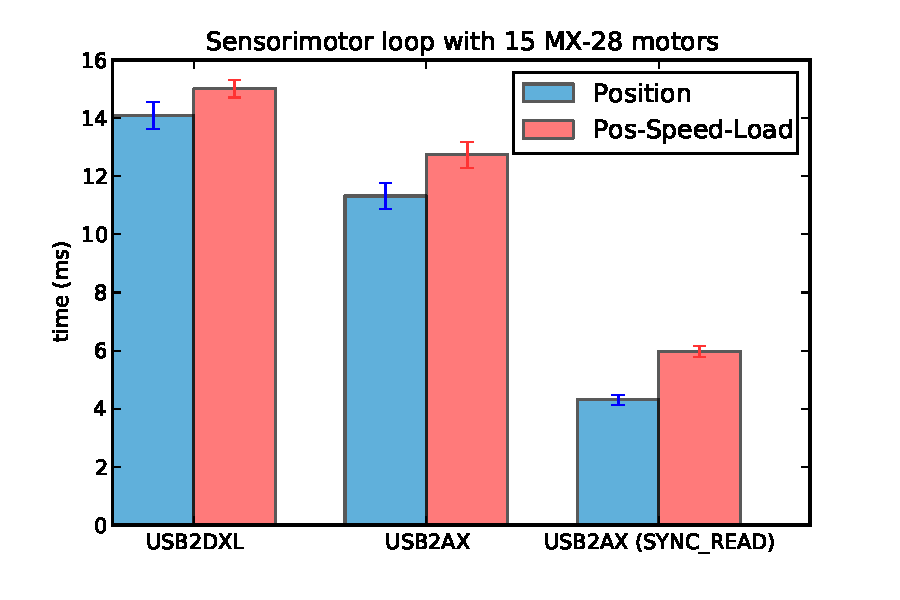
\includegraphics[width=0.7\linewidth]{motor-bench.pdf}
    \end{center}
    \caption{Caption here}
    \label{fig:figure1}
\end{figure}

This project has always been used on Poppy and greatly help us to both have a effective robot while keeping the room for electronic low.
Because the project is open hardware, we could have reuse it to embed it directly on a custom board so we can avoid having usb connectors.

\subsubsection{Arduino integration} % (fold)
As we explain in the section REF, the modularity of the Poppy electronics is achieved thanks to the use of Arduino environment. For the Arduino integration we decided to use the new Arduino Due based on the Atmel SAM3X8E ARM Cortex-M3 CPU. These board embeds both a powerful microcontroller (84 MHz 32-bit ARM core) and a large number of inputs/ouputs: 54 digital input/output pins (of which 12 can be used as PWM outputs), 12 analog inputs, 4 UARTs (hardware serial ports).



\subsection{Embedded computing module} % (fold)

The integration of a computing module is rather complex and not fundamental if the robot cannot walk for more than 5m, therefore the Poppy beta version was controlled using an external computer connected by USB.
However Poppy aims to become a shared research platform with people adressing challenge in which the embeded control can be necessary. Also as all user have a different computer configuration (Windows, MacOS and the plenty of Linux distribution), it is easier to maintain the control software if only one OS is used. Embedding a linux allows to have the control and ensure same performance for every Poppy.

Yet as I said previously, embedding control is complex. Indeed, the computer has to be small enough to fit inside the robot. With such size, where are mostly ARM based computer. Most of work are developed on x86 or 64 architecture and the switch to ARM architecture is not direct. Some software module used does not exist or are not optimized leading to big performance problems.

It is the case with one of the most famous micro-computer, the raspberry pi. The first trials we made using Pypot was really disappointing on the performance aspect. As we can see on the Figure Ref, it takes about 10-12 ms just to read and write a motor position (mostly computing) while it is only 2ms on a normal computer (mostly serial communication). Therefore we oriented our choice toward the Hardkernel Odroid U3 board (8\~12 times faster than the Raspberry Pi).

\begin{figure}[!h]
    \begin{center}
        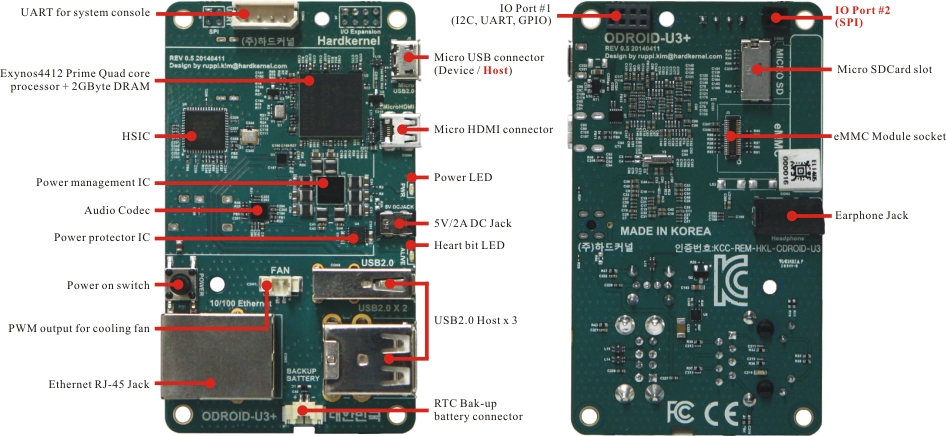
\includegraphics[width=\linewidth]{Odroid_U3.jpg}
    \end{center}
    \caption{Hardkernel Odroid U3 computer board}
    \label{fig:odroid_U3}
\end{figure}

The Hardkernel Odroid U3 (see \figurename~\ref{fig:odroid_U3}) is a low-cost (\$65) and powerful Linux computer embedding a 1.7GHz Quad-Core processor and 2GByte RAM while being very small (83 x 48 mm) and lightweight (48 grams) (see Tab.~\ref{tab:table_feet} for the detail of all specifications).

\begin{table}[!t]
    \begin{center}
        \begin{tabularx}{\linewidth}{r X}
        % \hline
        \textbf{Processor} & Samsung Exynos4412 Prime Cortex-A9 Quad Core 1.7Ghz with 1MB L2 cache\\
        \textbf{Memory} & 2048MB(2GB) LP-DDR2 880Mega data rate\\
        \textbf{3D Accelerator} & Mali-400 Quad Core 440MHz\\
        \textbf{Video} & supports 1080p via HDMI cable(H.264+AAC based MP4 container format)\\
        \textbf{Video Out} & micro HDMI connector\\
        \textbf{Audio} & Standard 3.5mm headphone jack HDMI Digital\\
        \textbf{LAN} & 10/100Mbps Ethernet with RJ-45 Jack ( Auto-MDIX support)\\
        \textbf{USB2.0 Host} & High speed standard A type connector x 3 ports\\
        \textbf{USB2.0 Device} & ADB/Mass storage(Micro USB), Host mode is possible if the PCB Rev is 0.5 or higher.\\
        \textbf{Display} & HDMI monitor\\
        \textbf{IO Port} & GPIO, UART, I2C, SPI(Board Revision 0.5 or higher)\\
        \textbf{Storage (Option)} & MicroSD Card Slot eMMC module socket\\
        \textbf{Power (Option)} & 5V 2A Power\\
        \textbf{System Software} & Linux : Xubuntu 13.10 or latest version Android : u-boot 2010.12, Kernel 3.0.x, Android 4.x  Full source code is available now.\\
        \textbf{PCB Size} & 83 x 48 mm\\
        \textbf{Weight} & 48g including the heat sink\\
         & \\
        % \hline
        \end{tabularx}
        \caption{Odroid U3 Linux computer detailed specifications}
        \label{tab:table_feet}
    \end{center}
\end{table}

Among the plug-n-play small computers, the Odroid U3 is currently the most suitable board for our application according to the size, the computing power and the I/O positions.
Yet as we will explain in the limitations (see section REF), this solution is still not perfectly satisfying and the use of plug'n'play computer raises a lot of integration problem.

\subsection{Display} % (fold)

The video out port on all new mini computer boards such as Raspberry Pi, Beagle board or Odroid boards is HDMI port. Finding small screen (< 7inch) compatible with HDMI input is really hard and currently only one project exists.The manga-screen (see \figurename~\ref{fig:manga-screen}) is a open source (CC-BY-SA\footnote{see REF}) multi purpose, HDMI compatible LCD screen. This board is developed by Elias Bakken and works with a 4.3 inch screen (480x800px) made by Sharp\footnote{Sharp LQ043Y1DX07}.

\begin{figure}[h]
\centering
    \subfloat[][]{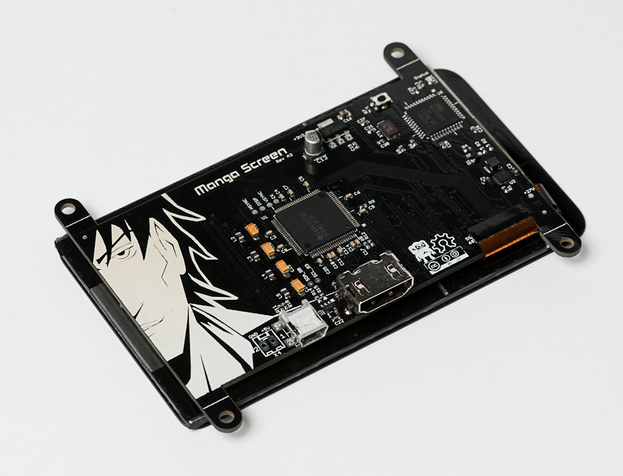
\includegraphics[height=4.9cm]{manga-screen.png}}
    \hfil
    \subfloat[][]{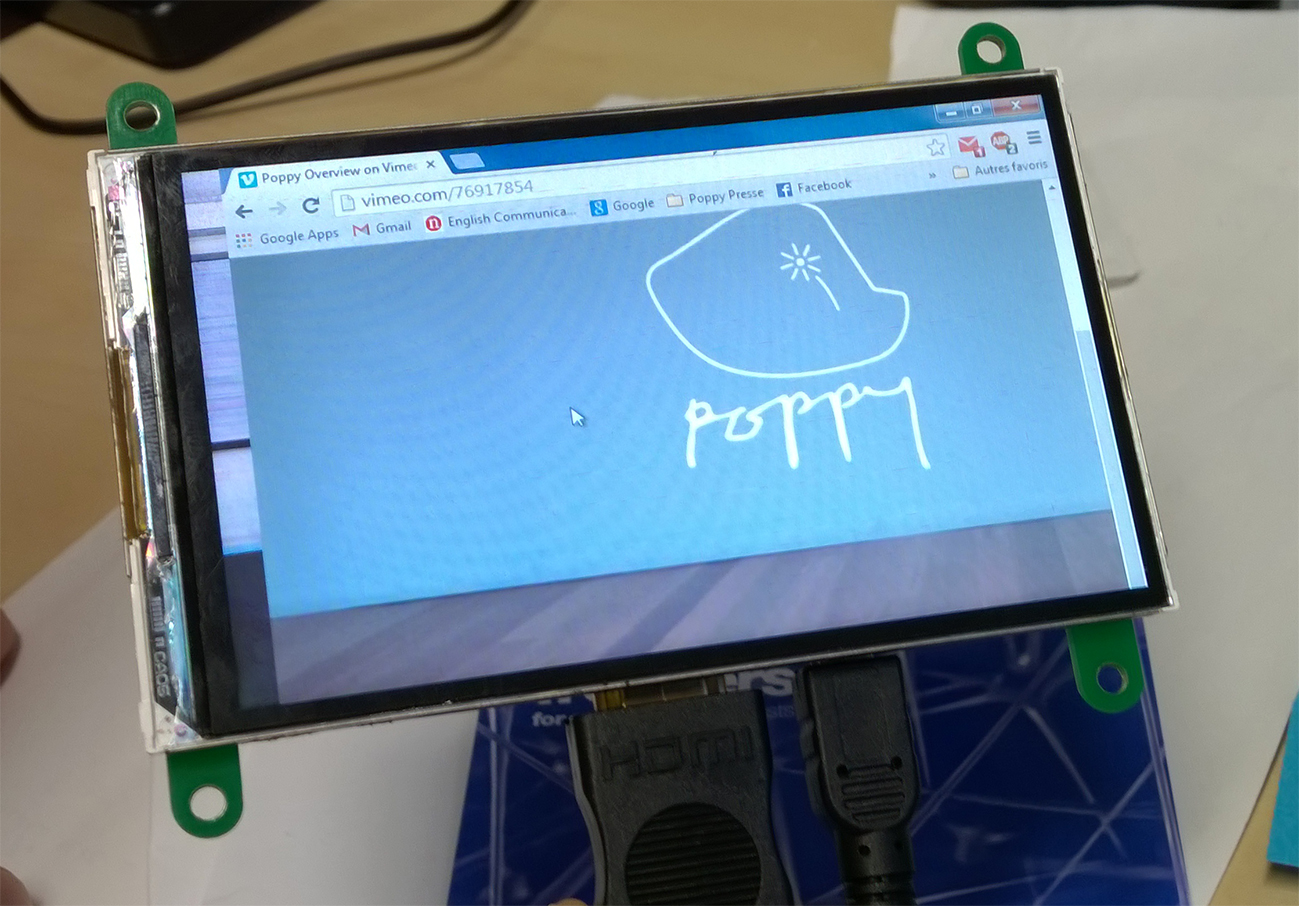
\includegraphics[height=4.9cm]{poppy_screen.jpg}}
    \caption{}
    \label{fig:manga-screen}
\end{figure}

The integration of a led matrix panel would be easier but it would require to create driver for the display.
Using a HDMI display connected to a Linux computer allows user to easily display information or animation on the screen like if it was on their monitor. Therefore they are free to use any tools they like such as Processing, OpenGL, VLC or whatever. This flexibility would not be possible with a matrix led panel which could basically only be used by Arduino.

\subsubsection{Alimentation} % (fold)
\label{ssub:alimentation}

Work in progress.

% subsubsection alimentation (end)

\subsubsection{The battery issue} % (fold)
In the current design electronic architecture we did not include a battery. The main reason is the fact Poppy is not yet able to walk by itself so being energetically autonomous is not a high-priority.

Another issue associated with the batteries is the mass. A 3.6V battery cell weights around 45 grams and we need at least 4 cells to supply the 12V needed for Poppy, a 14,4V pack weights almost 200 grams (see \figurename~\ref{fig:battery_specs}). For comparison a MX-28 Dynamixels weights 72grams so with a battery weigths approximately the same mass as 3 motors.

Finally the overall size of such cell is rather big with 18mm x 65mm (see \figurename~\ref{fig:battery_size})

\begin{figure}[tb]
\centering
    \subfloat[][]{\label{fig:battery_size}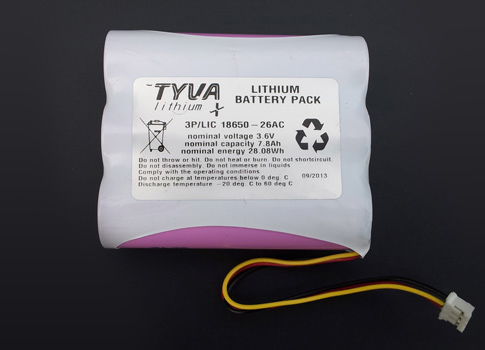
\includegraphics[height=3.5cm]{tyva_battery_pack.jpg}}
    \hfil
    \subfloat[][]{\label{fig:battery_specs}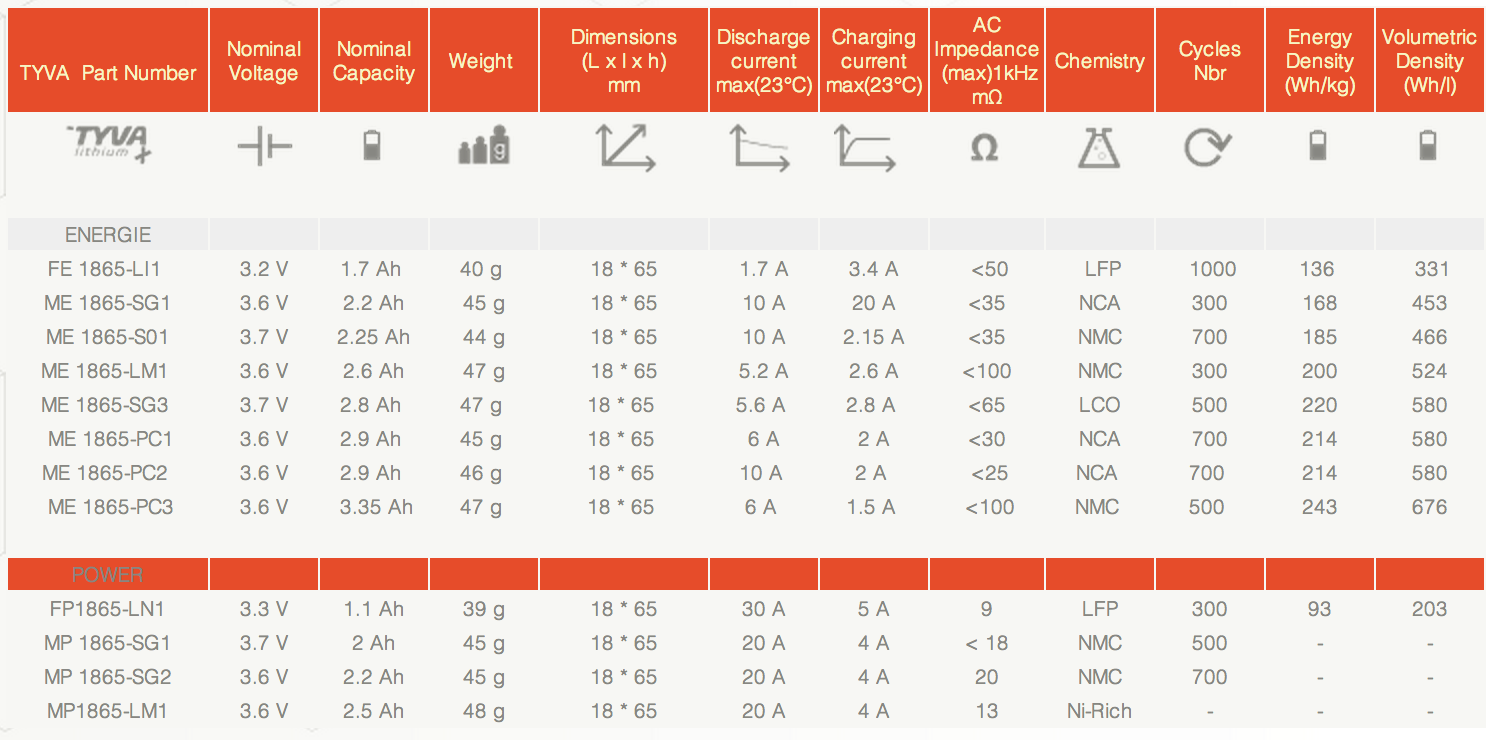
\includegraphics[height=4cm]{tyva_batteries.png}}\\
    \caption{}
    \label{fig:tyva_batteries}
\end{figure}



\section{Head aesthetic design} % (fold)

Lot of effort have been put in the design and aesthetic of Poppy's head (see \figurename~\ref{fig:poppy_beta_head}), both its identity and main communication apparatus.
On an aesthetic point of view, its design was inspired of course by existant robots, but also by animals, objects and arts. The main inspiration insight are displayed as a board on the \figurename~\ref{fig:head_inspiration}. We tried to make to achieve a design cute, expressive and among all simple.

\begin{figure}[p]
    \begin{center}
        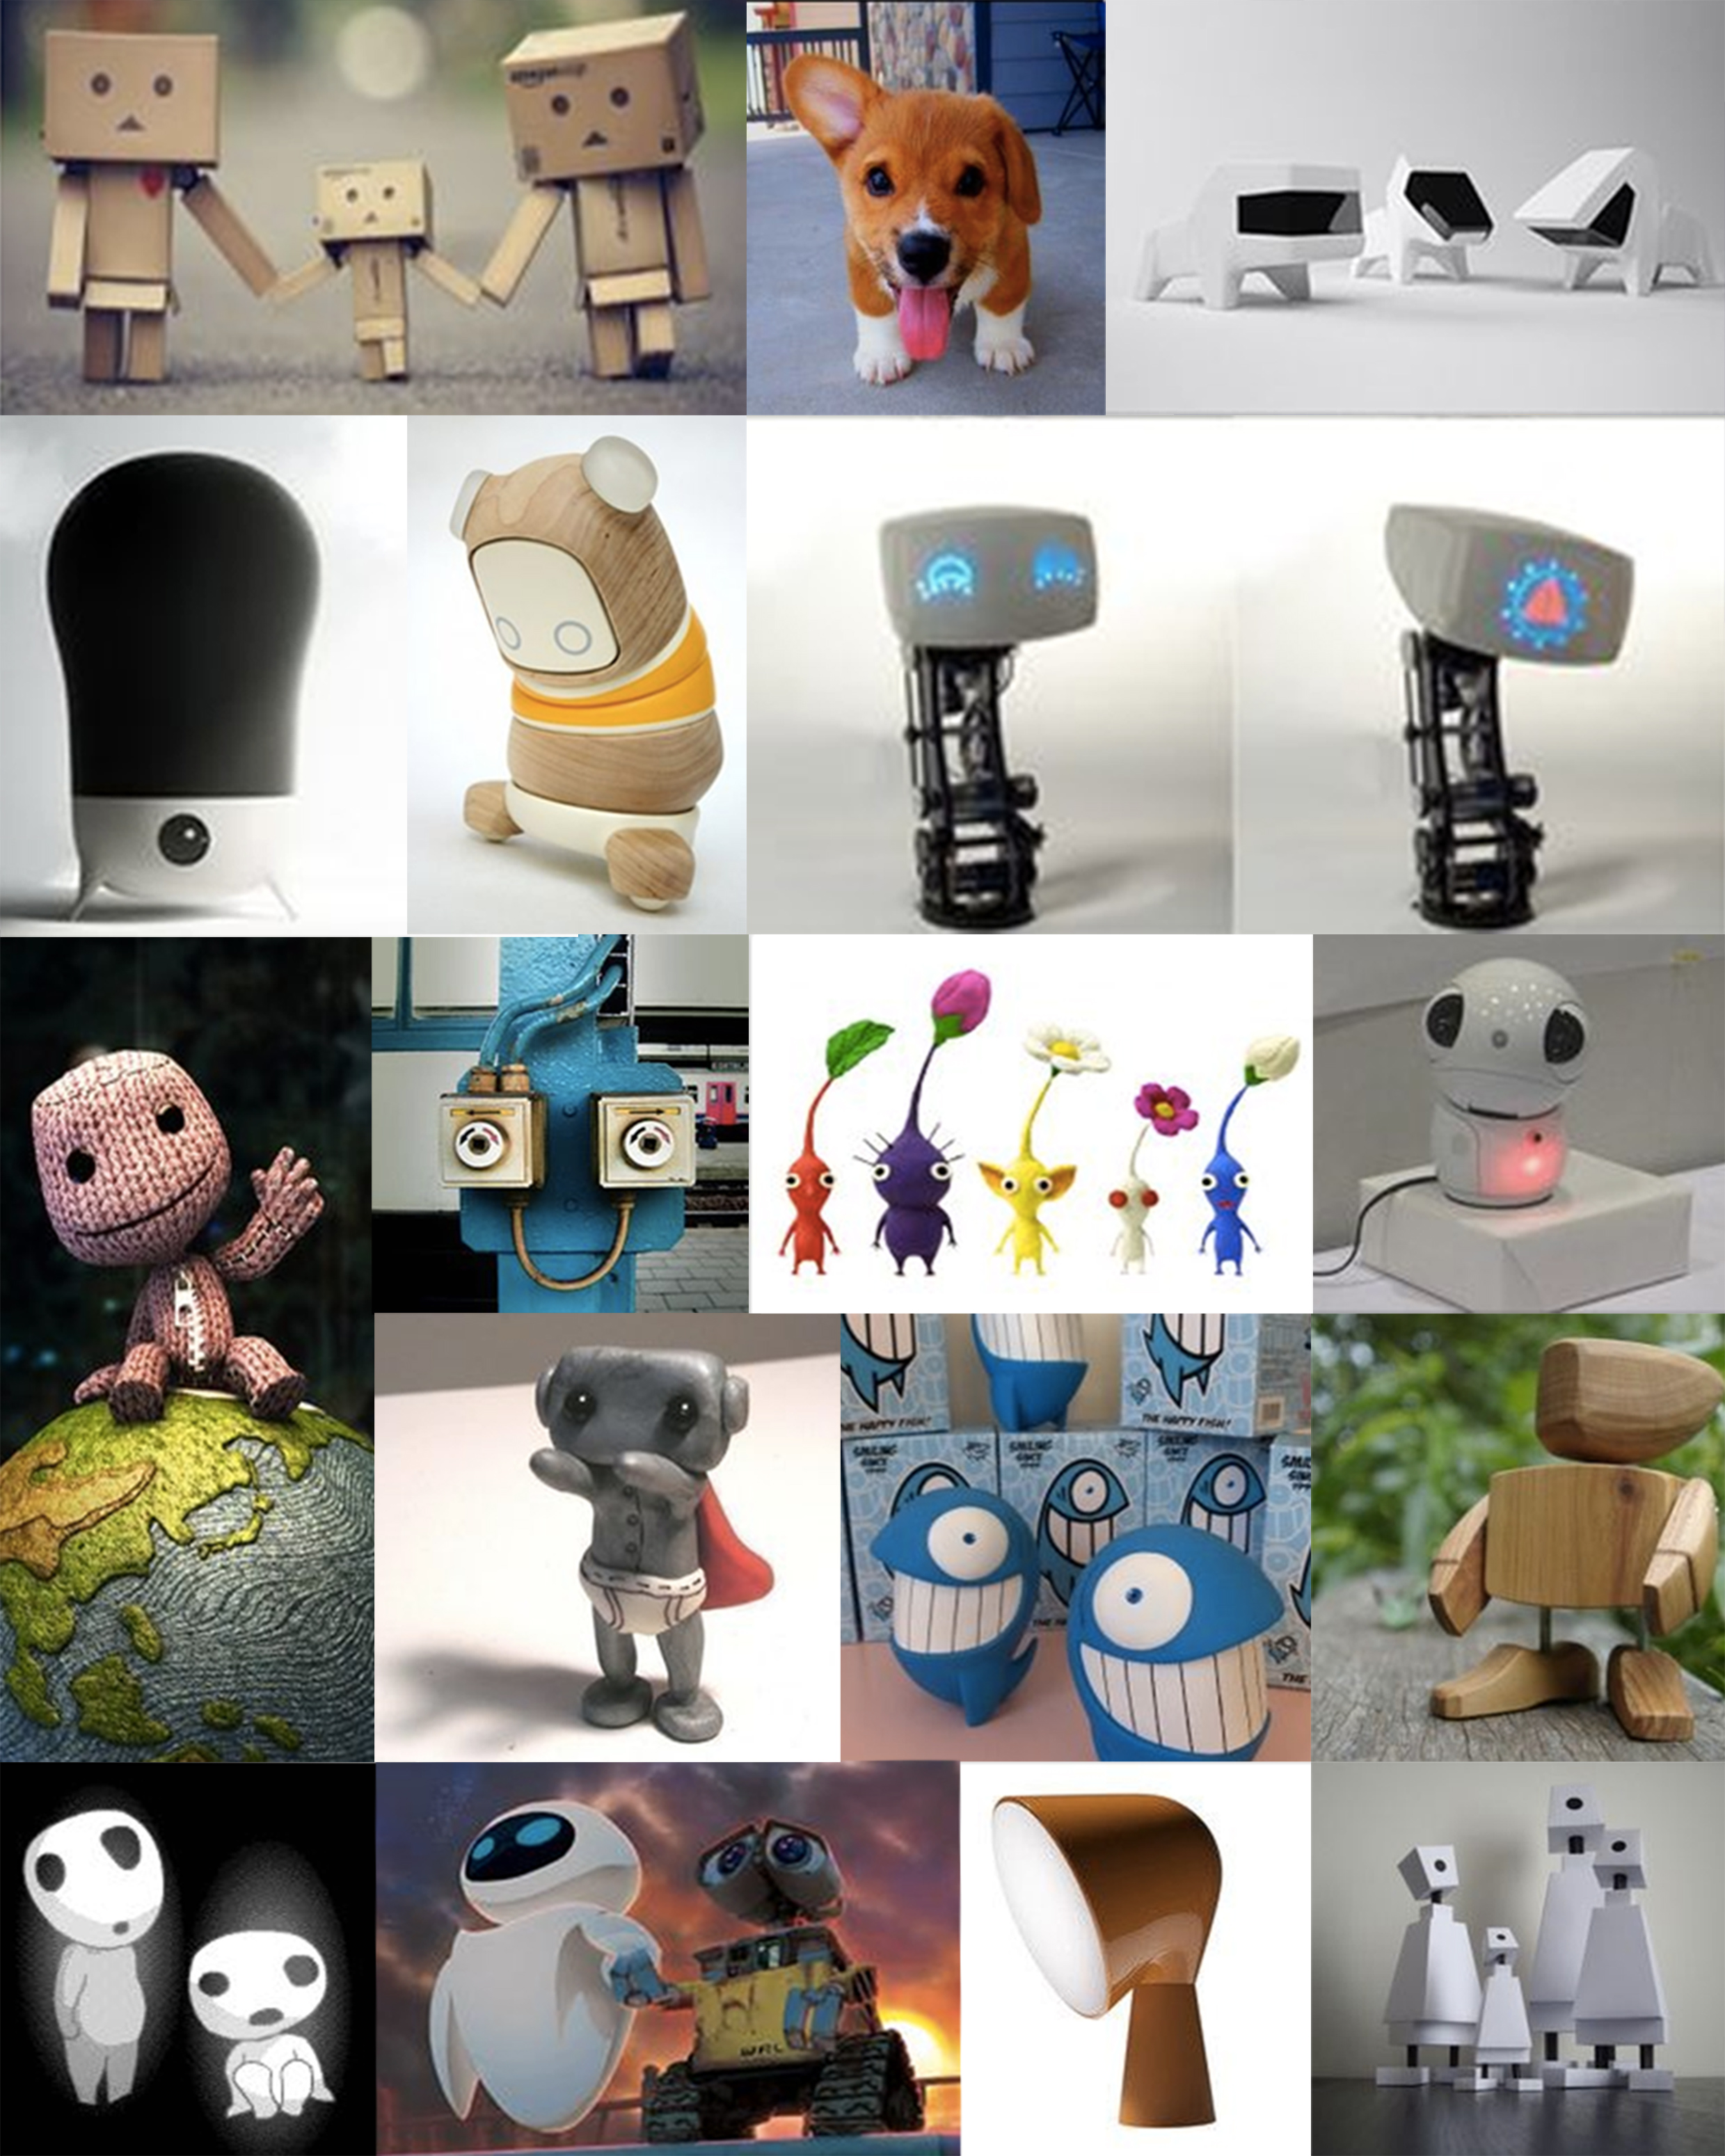
\includegraphics[width=\linewidth]{head_inspiration.jpg}
    \end{center}
    \caption{Complete board available on pinterest \url{http://www.pinterest.com/matthieulapeyre/robot/}}
    \label{fig:head_inspiration}
\end{figure}

Yet because of the multi-articulated vertebral column, Poppy has only free room in the head to embed all electronics components needed. Therefore strong technical constraints were imposed because the head has to embed all electronic architecture plus the communication sensorimotor apparatus composed by a wide 4.3" screen, cameras, audio.
This components strongly constraints the design of the robot. Especially the screen, which requires a large flat part on the face. Obtaining a nice and rounded head shape with such constraints were rather difficult and require several iterations before obtaining a first correct finish (see \figurename~\ref{fig:poppy_beta_head}).

% This process involved first few sketches that gave the main idea of the desired design. Yet the transfer to CAD modeling was quite complex, this kind of shape are rather difficult to design using parametric tools.

\begin{figure}[p]
\centering
    \subfloat[][]{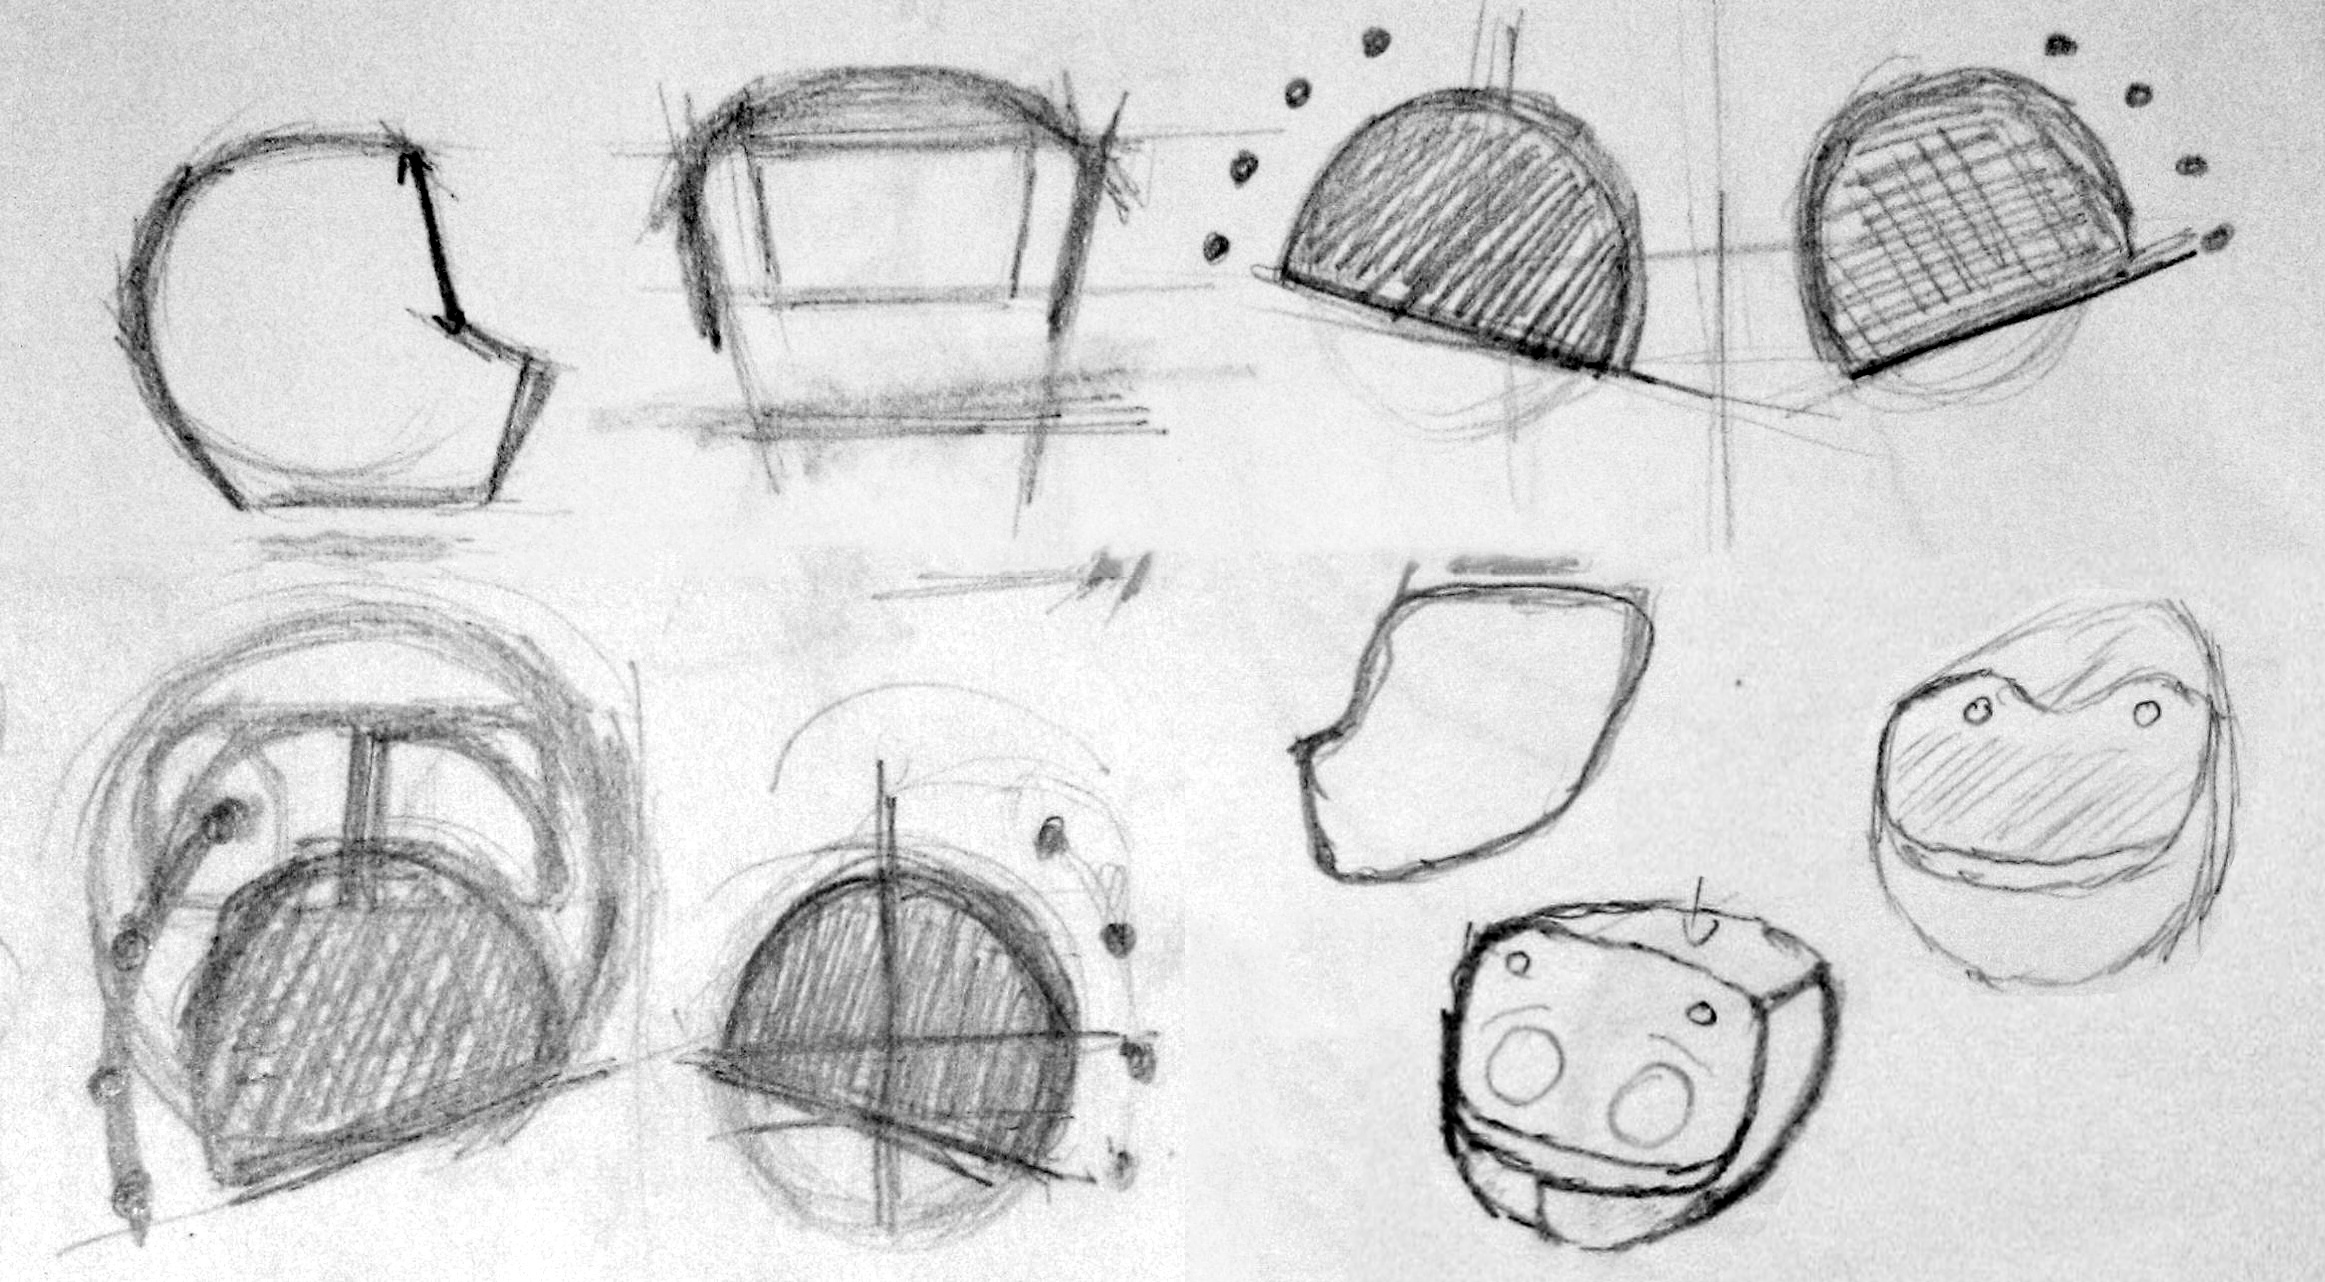
\includegraphics[height=4.5cm]{first_sketch.jpg}}
    \hfil
    \subfloat[][]{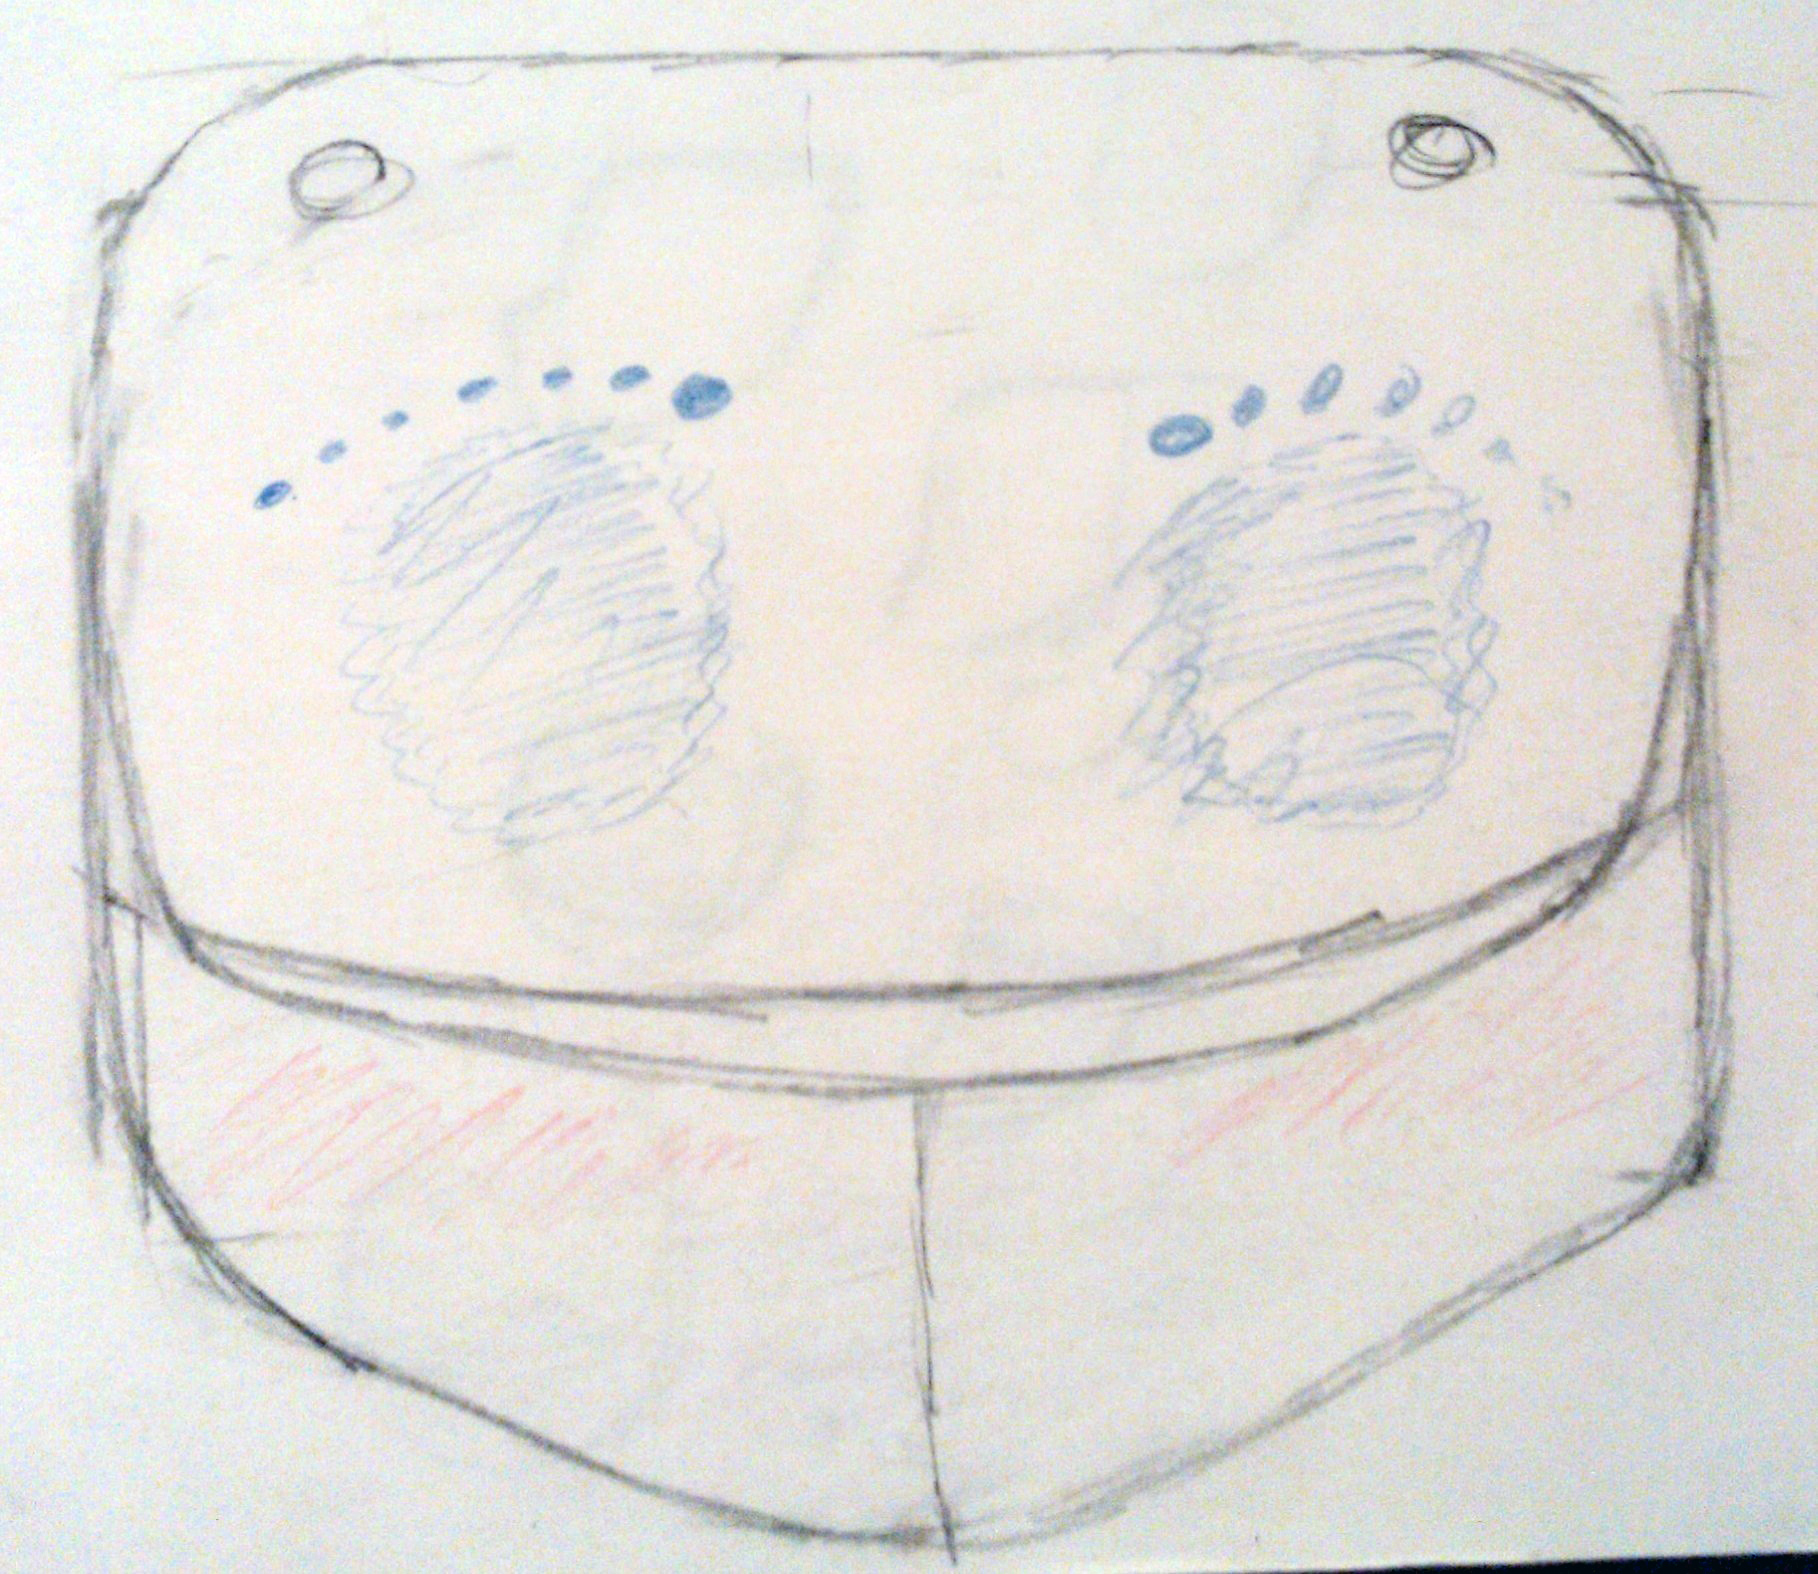
\includegraphics[height=4.5cm]{poppy_head_sketch.jpg}}
    \newline
    \subfloat[][First clay sculpture]{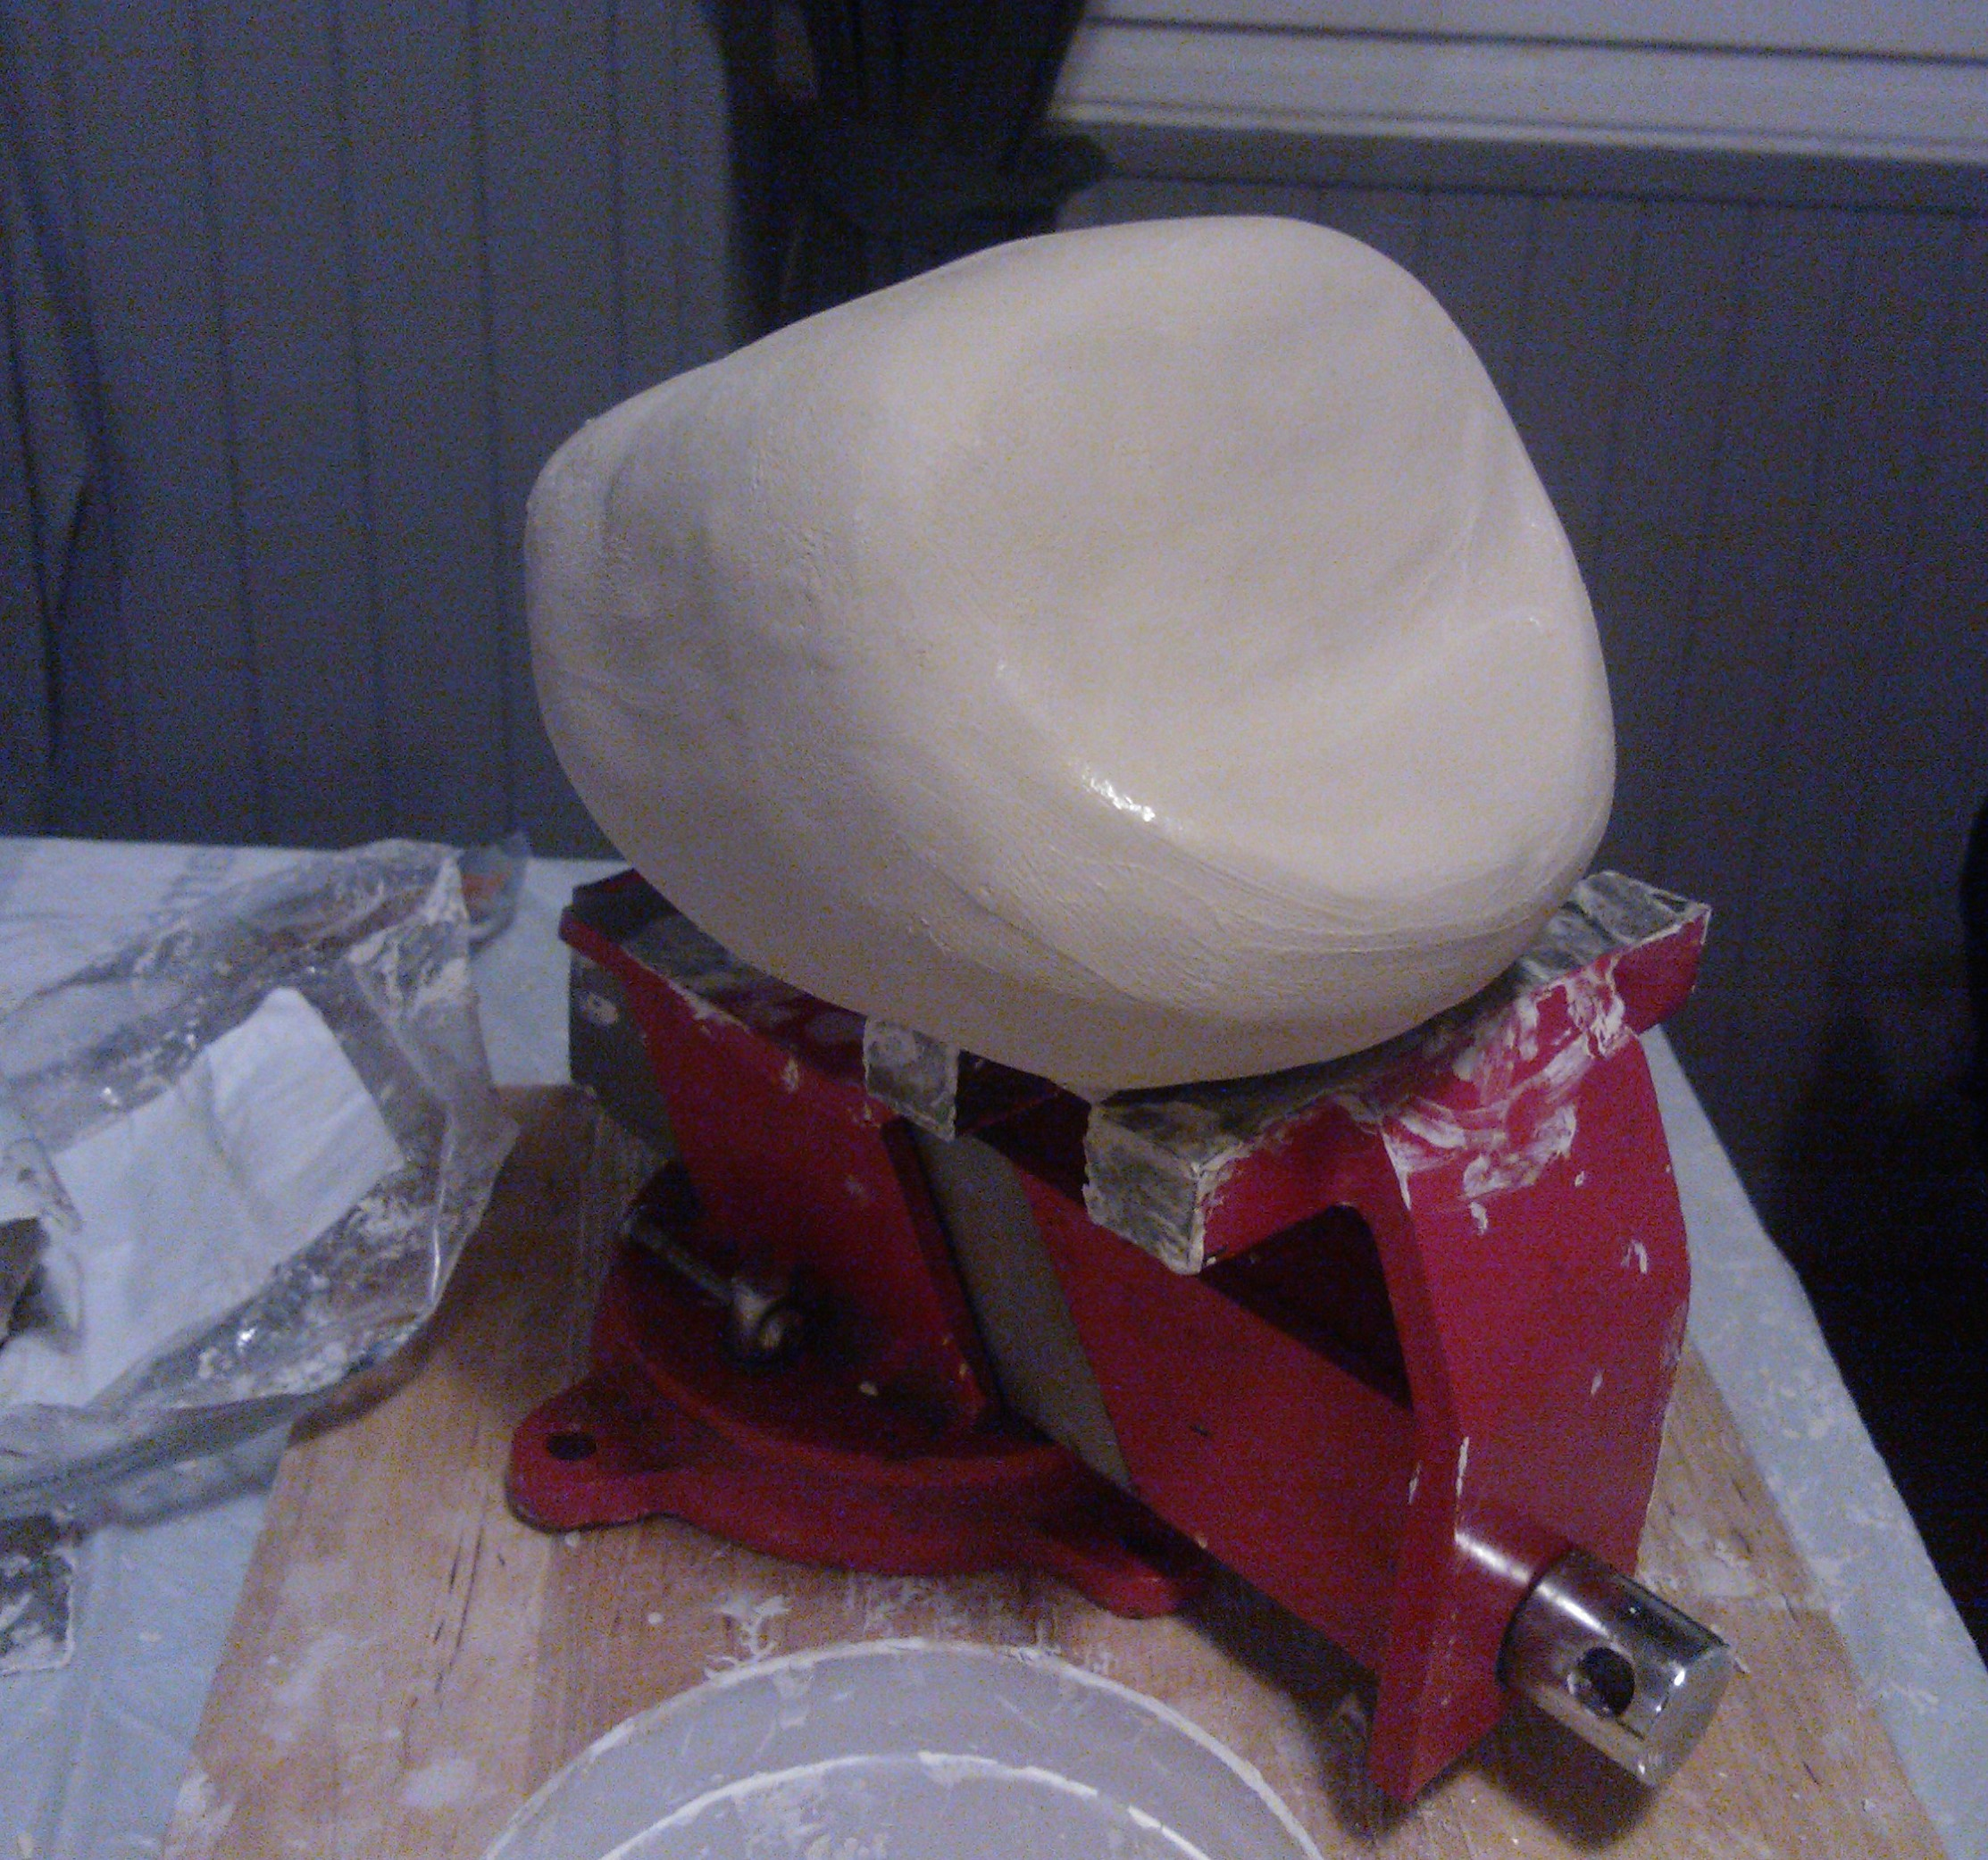
\includegraphics[height=5.5cm]{first_poppy_clay.jpg}}
    \hfil
    \subfloat[][First CAO model]{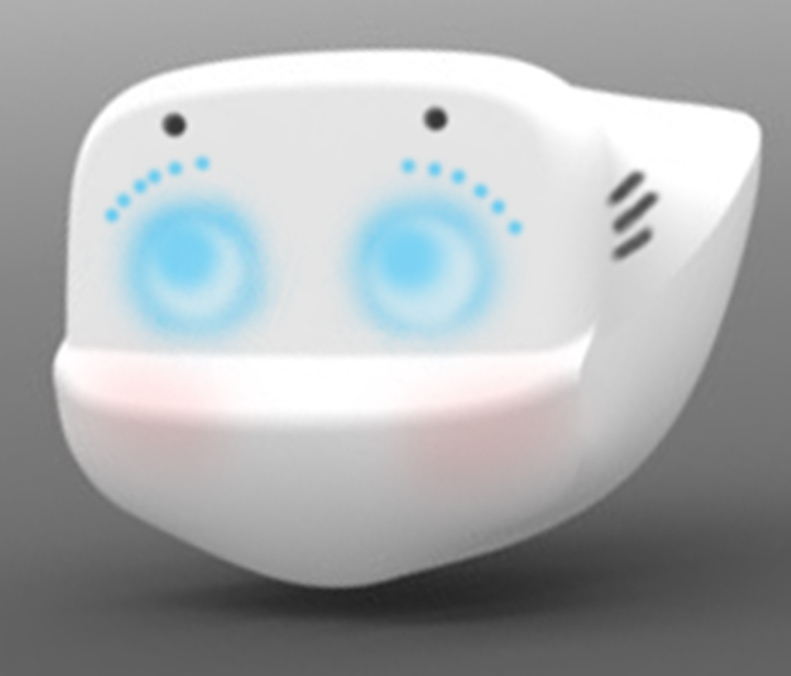
\includegraphics[height=5.5cm]{head_first_trial.jpg}}
    \newline
    \subfloat[][Poppy beta]{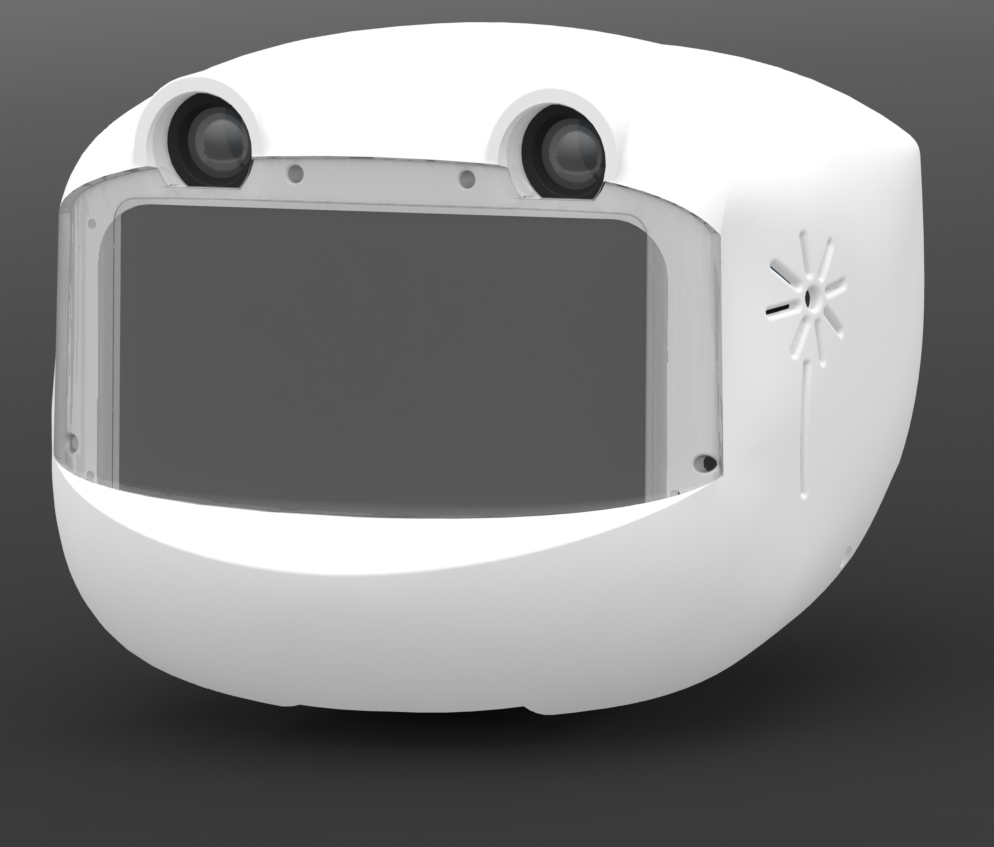
\includegraphics[height=5.5cm]{head_beta.jpg}}
    \hfil
    % \subfloat[][The first assembly]{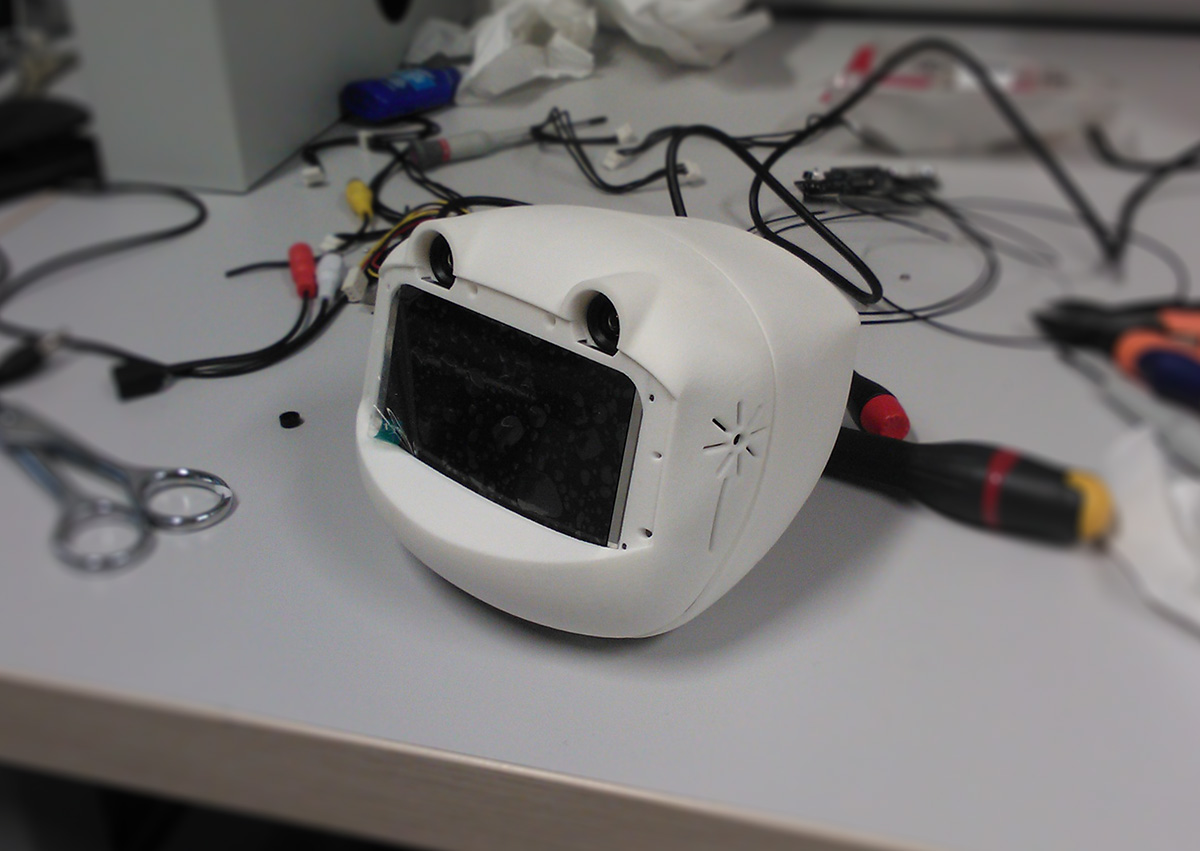
\includegraphics[height=5.5cm]{head_beta_assembled.jpg}}
    % \hfil
    \subfloat[][Screen powered on with basic eyes display]{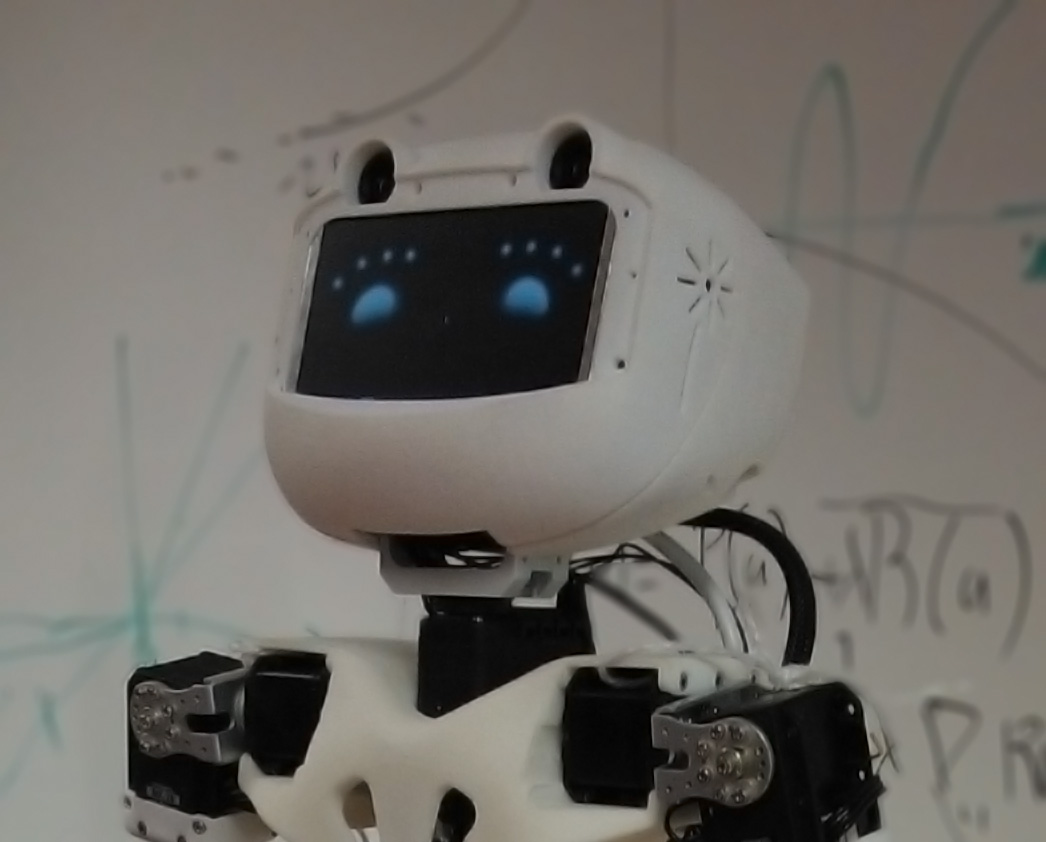
\includegraphics[height=5.5cm]{poppy_beta_eyes.jpg}}
    \caption{Evolution of Poppy head from the first sketches to the Poppy beta version.}
    \label{fig:head_sketch}
\end{figure}


However, in the first beta version showed here, there is a major design error. Indeed my desire was to have a screen to create and explore freely expressive eyes but the use of two visible cameras changed the way people saw Poppy's head. Of course, people seeing 2 cameras considers they are the eyes of the robot and therefore extrapolate that the screen may be the mouth.

We are working on this issue by replacing the two big camera by a small one with a pinhole lens, which can be hidden on the Poppy face see \figurename~\ref{fig:poppy_head_v1}.

\begin{figure}[tb]
\centering
    % \subfloat[][Mix between Poppy beta 3D printed head and clay sculpture]{\includegraphics[height=5cm]{second_poppy_clay.jpg}}
    % \newline
    \subfloat[][Poppy 1.0]{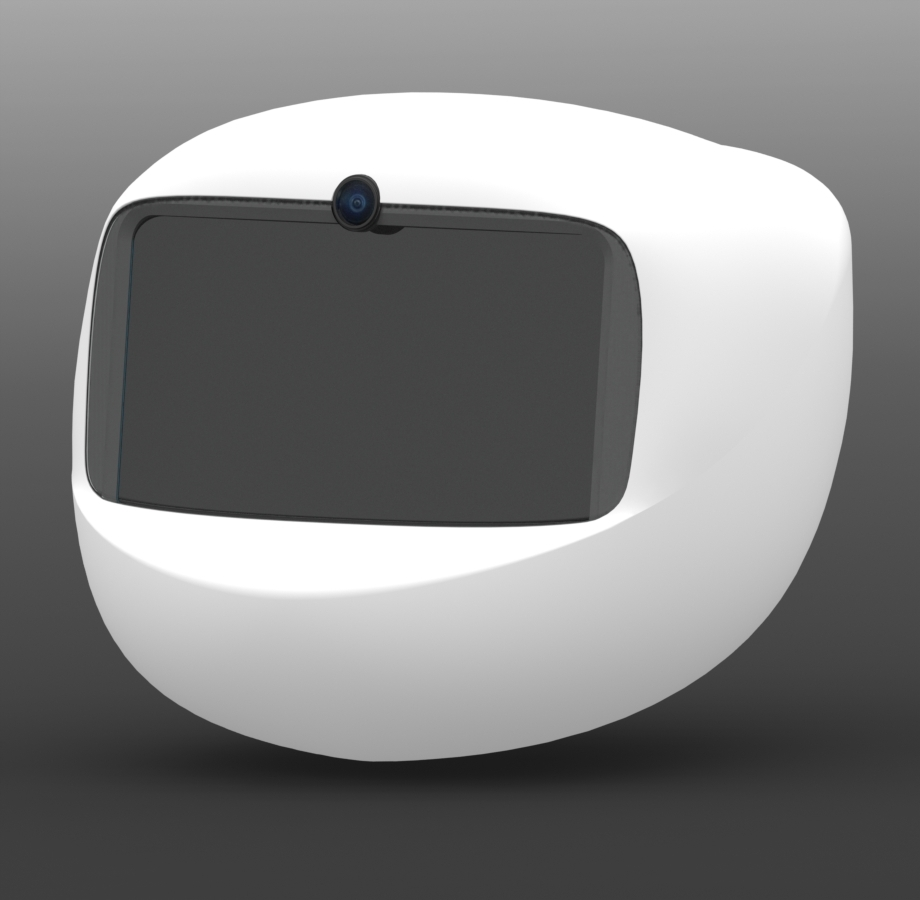
\includegraphics[width=0.5\linewidth]{poppy_v1_head.jpg}}
    \caption{}
    \label{fig:poppy_head_v1}
\end{figure}




\section{Conclusion} % (fold)


\subsection{Electronic limitations} % (fold)

The electronic we developed is compatible with the exploration of morphology for sensory space because it has a lot of I/O ports to extend Poppy's sensorimotor space. Yet it has several limitations which make the final solution unsatisfying.

Commonly used electronic components are not designed for robotic integration but rather for building small personal computers. Thus even if the electronic boards are often quite smalls, they have big common connectors such as USB, HDMI, Ethernet which are of course never placed exactly where it should be for the integration in the robot.
Above all, cable are really annoying, they take surprisingly a lot of room (connector size, the wire length and they are heavy) while being totally useless for our applications.

Also the size of the IO Board is finally pretty big, more than expected and while it is still compatible with the Poppy design, it is too big with a too weird shape to be relevant for other open source project.

Great open source projects keep their work modular so other project can use directly one or several modules. Therefore the IO Board is not compatible with such principle and is currently under evolution toward the building of a modular Poppy electronics (we will discuss this new version in the discussion see REF). Yet this IO Board was the first electronic board developed in the Poppy project and the experience we acquire a better understanding of electronic integration. If we have to do it today we would make the same mistakes.

In particular, even if we tried to remove most of the necessary cables, we saw it is still complicated to make integration. We really have to develop board which do not require any wire at all.

Actually, I spent more time looking for the fitting cable on the web than thinking about the electronical architecture. The wire-problem is often under-estimated and therefore begin one the biggest problem for robotic. We experienced the same issue during the ergo-robot experiment and during the use of Poppy with artists (see chapter REF). SO basically, the wire problem is one of the most underrated issue.


